\documentclass{beamer}
\usetheme{Madrid}
\usecolortheme{crane}
\usepackage{animate}
\usepackage{graphicx}
\usepackage{amsmath}
\usepackage{amsfonts}
\usepackage{amssymb}
\usepackage{amsthm}
\usepackage{complexity}
\usepackage{caption}
% \usepackage{subcaption}
\usepackage{enumerate}
\usepackage{enumitem}
\usepackage{array}   % for \newcolumntype macro
% \usepackage{refcheck}
\newcolumntype{L}{>{$}l<{$}} % math-mode version of "l" column type
\newcolumntype{R}{>{$}r<{$}} % math-mode version of "r" column type
\newcolumntype{C}{>{$}c<{$}} % math-mode version of "c" column type
% %%%theoerms, etc%%%%
\newtheorem{thm}{Theorem}
\newtheorem{prob}{Problem}
\newtheorem{lem}{Lemma}
%%%%%%%%custom commands
\newcommand{\ith}{i^\text{th}}
\newcommand{\jth}{j^\text{th}}
\newcommand{\kth}{k^\text{th}}
\newcommand{\NN}{\mathbb{N}} %  set of natural numbers
\newcommand{\ZZ}{\mathbb{Z}} %  set of integer number
\newcommand{\RR}{\mathbb{R}} %  set of real numbers
\newcommand{\SH}{\mathbb{S}} %  set of unit vectors
\newcommand{\HH}{{\mathcal{H}}} %  Calligraphic H
\renewcommand{\PP}{{\mathcal{P}}} %  Calligraphic P
\newcommand{\DD}{{\mathcal{D}}} %  Calligraphic D
\newcommand{\QQ}{{\mathcal{Q}}} %  Calligraphic D
\newcommand{\FF}{{\mathcal{F}}} %  Calligraphic D
\newcommand{\bbH}{{\mathbb{H}}}
\newcommand{\bbR}{{\mathbb{R}}}
\newcommand{\bbP}{{\mathbb{P}}}
\newcommand{\bbZ}{{\mathbb{Z}}}
\newcommand{\bbC}{{\mathbb{C}}}
\newcommand{\bbQ}{{\mathbb{Q}}}
\newcommand{\bbA}{{\mathbb{A}}}
\newcommand{\bbF}{{\mathbb{F}}}
\newcommand{\bbh}{{\mathbb{H}}}
\newcommand{\bbr}{{\mathbb{R}}}
\newcommand{\bbp}{{\mathbb{P}}}
\newcommand{\bbz}{{\mathbb{Z}}}
\newcommand{\bbc}{{\mathbb{C}}}
\newcommand{\bbq}{{\mathbb{Q}}}
\newcommand{\bba}{{\mathbb{A}}}
\newcommand{\bbf}{{\mathbb{F}}}
\newcommand{\bbn}{{\mathbb{N}}}
\newcommand{\bbN}{{\mathbb{N}}}
\newcommand{\lr}[1]{\left( #1 \right)}


\title[Planar Configuration Spaces]{Planar Configuration Spaces }
\subtitle{of Disk Arrangements and Hinged Polygons}
\author{Clinton Bowen}
\institute
{
  Cal State Northridge
}
\date
{December 6, 2016}
\subject{Mathematics}
\begin{document}
\frame{\titlepage}
	
\begin{frame}\frametitle{Motivation: Deciding Realizability of Polygonal Linkages}
	\begin{prob}
	Decide whether a polygonal linkage whose hinge graph is a \textit{tree} can be realized?
	\end{prob}
% \begin{columns}[c] % the "c" option specifies center vertical alignment
%   \column{.5\textwidth};lk;klj % column designated by a command
%    % \begin{itemize}
%             % \item[*]  A polygonal linkage is an ordered pair $\left(\PP,\HH \right)$ where $\PP$ is a finite set of polygons and $\HH$ is a finite set of hinges.
%             % \item[*]  A \textit{hinge} $h\in \HH$ corresponds to two or more points on the boundary of distinct polygons in $\PP$. 
%     % \end{itemize}
%   \column{.5\textwidth}
%   ;lkhlk
    \begin{minipage}{\linewidth}
        \begin{center}
            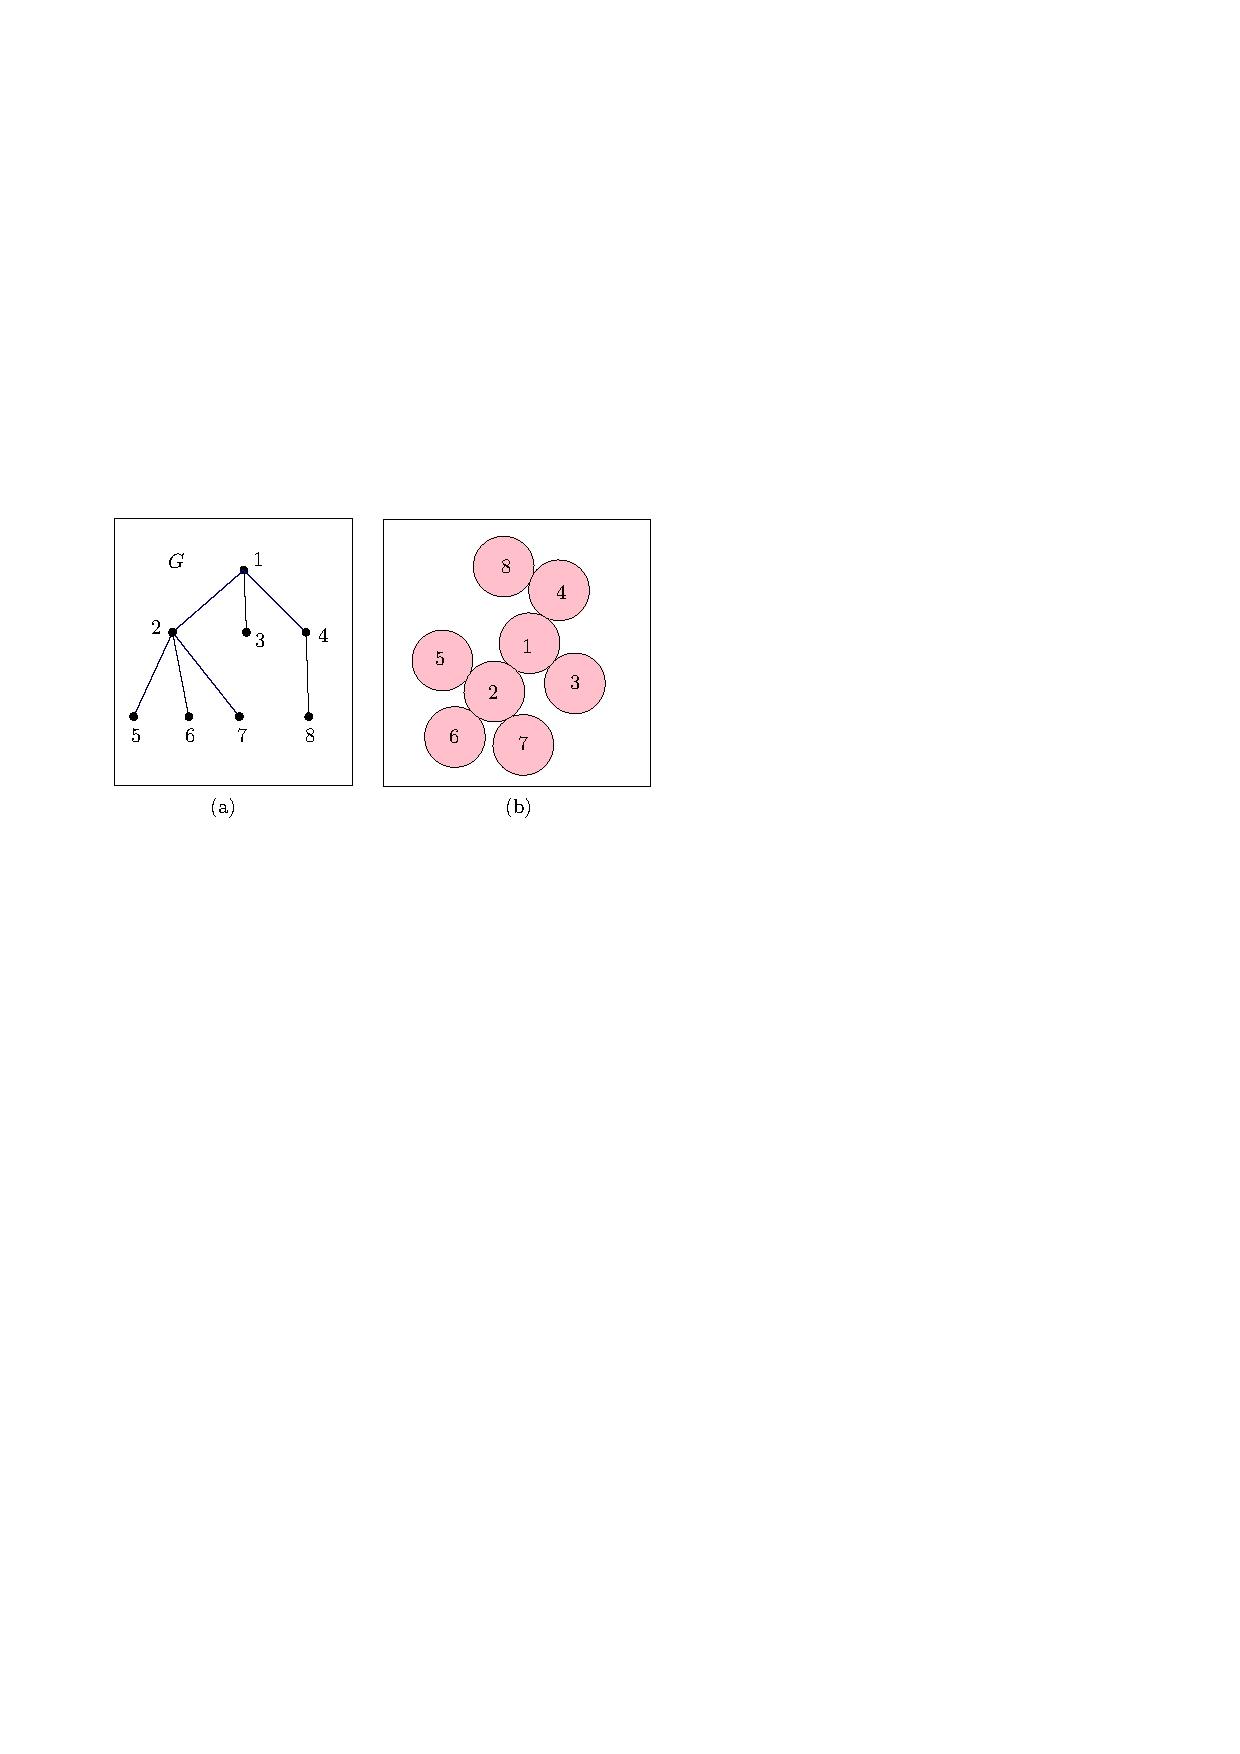
\includegraphics[width=\linewidth]{graphics/fig3++.pdf}
        \end{center} 
    \end{minipage}
%   \end{columns}
\end{frame}

\begin{frame}\frametitle{Motivation: Polygonal Linkages}
    \begin{columns}[c]
    \column{.5\textwidth}
        \begin{itemize}
        	\item[*] The figure on the top shows a realizable polygonal linkage.
        	\item[*] The firgure on the bottom shows a polygonal linkage that is not realizable.
    \column{.5\textwidth}
        \begin{minipage}{\linewidth}
            \begin{center}
            
\includegraphics[width=.9\textwidth]{graphics/hingeOnThreeDistinctPolygons.pdf}\label{gfx:hingeOnThreeDistinctPolygons.pdf}\vspace{.25in}
            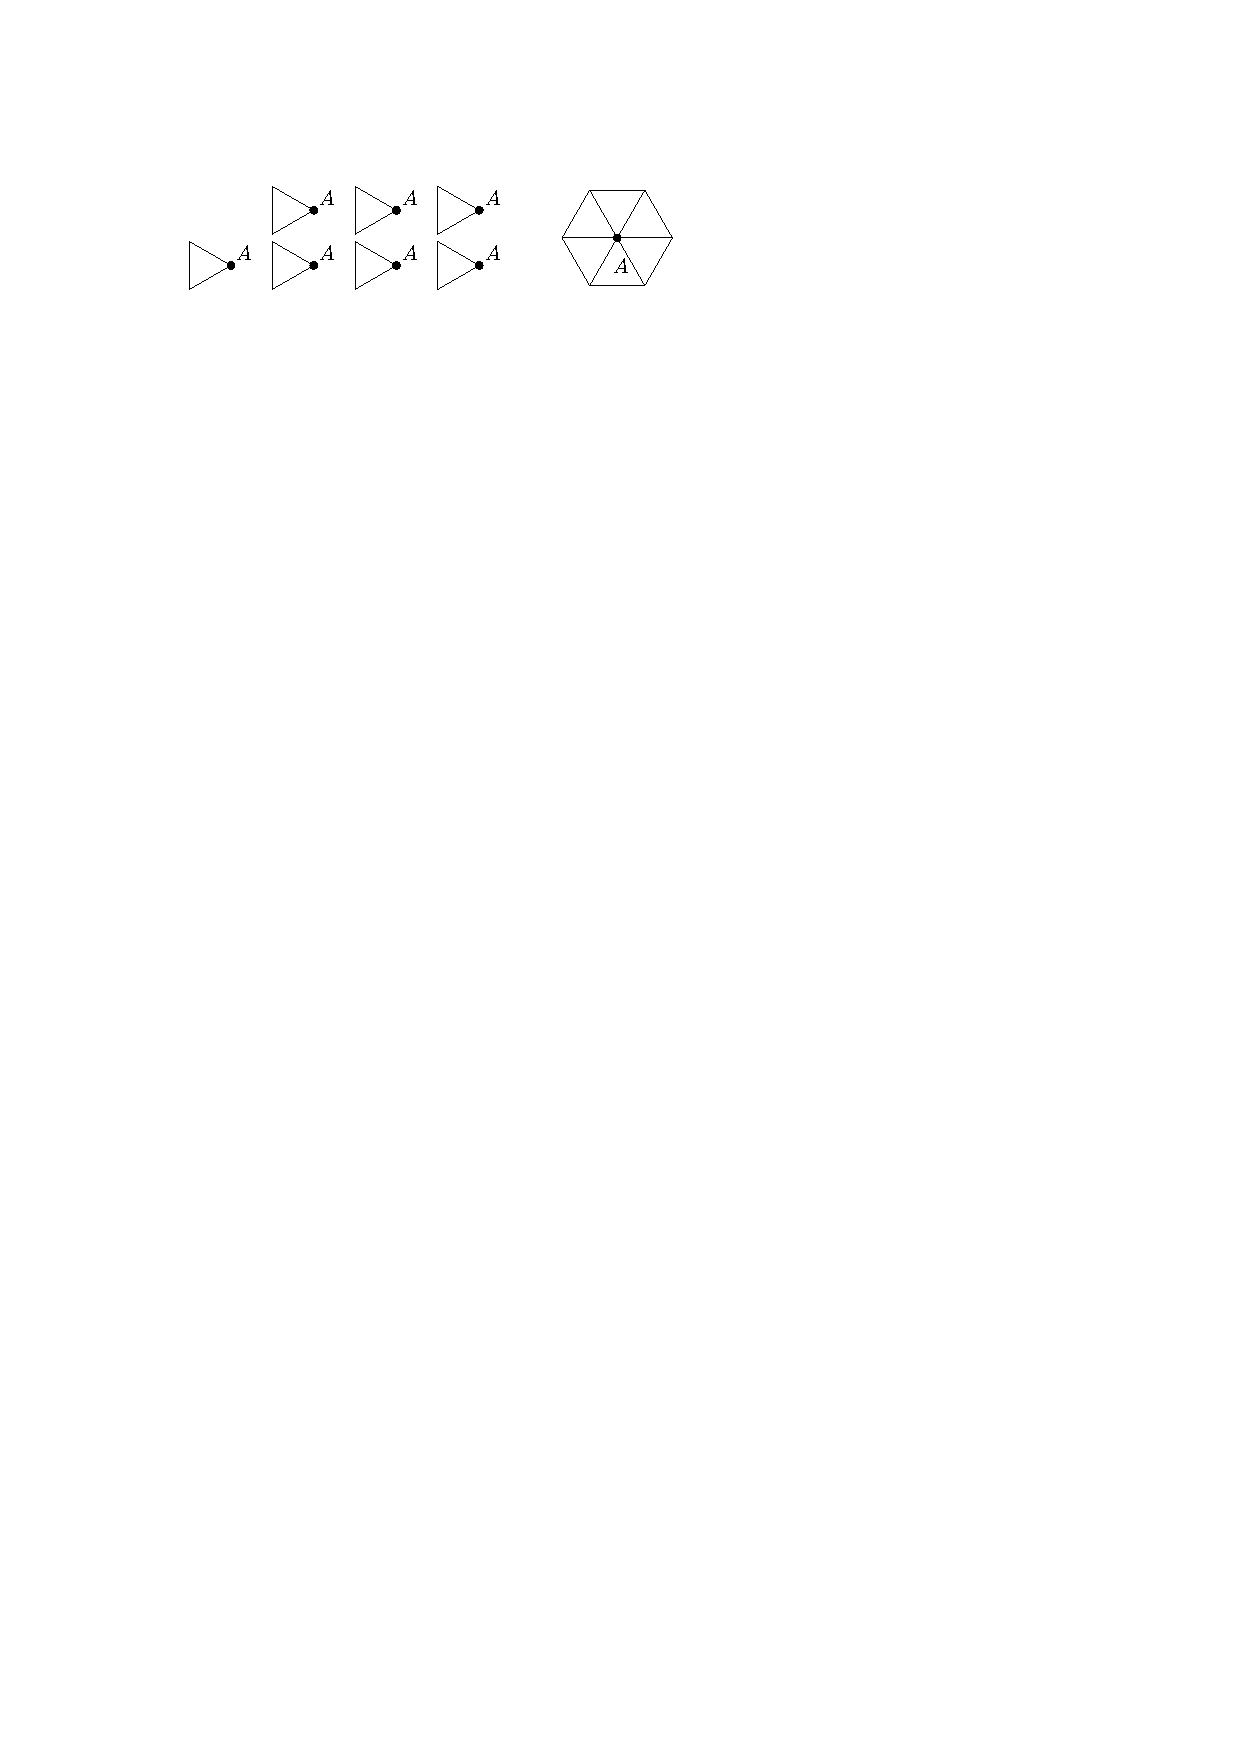
\includegraphics[scale=1]{graphics/Problem1.pdf}
            \label{fig:problem1}
            \end{center}
        \end{minipage}
    \end{columns}
\end{frame}

\begin{frame}\frametitle{Motivation: Hinged Dissection}
    \begin{columns}[c]
    \column{.5\textwidth}
        \begin{itemize}
            \item[*] \textit{Haberdasher Problem}: Can a square and an equilateral triangle of the same area have a common dissection into four pieces?
            \item[*]  \textit{Hilbert's Third Problem}: given any two polyhedra of equal volume, is it always possible to cut the first into finitely many polyhedral pieces which can be reassembled to yield the second?  
        \end{itemize}
  \column{.5\textwidth}
  \begin{minipage}{\linewidth}
    \begin{center}
    \animategraphics[loop,controls,width=\linewidth]{12}{graphics/hingedanimation-}{0}{107}
    \end{center}
  \end{minipage}
  \end{columns}
    \footnotetext{Source: Wikipedia}
\end{frame}

\begin{frame}
  \frametitle{Motivation: Protein Folding}
  Protein folding is the process in which a protein chain acquires its 3-dimensional structure.
  \begin{columns}[c] 
  \column{.5\textwidth} 
   \begin{itemize}
    \item[*] Proteins in an organism fold into a specific geometric pattern (sometimes referred as its \textit{native state}).
    \item[*]  Geometric patterns can determine a protein's function and behavior.
   \end{itemize}
  \column{.5\textwidth}
     \begin{minipage}{\linewidth}
        \begin{center}
        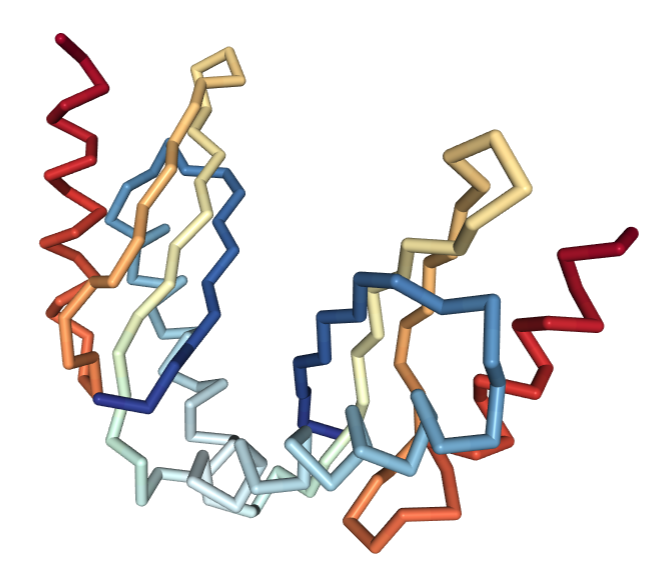
\includegraphics[width=\linewidth]{graphics/5HHB.png}
        \end{center} 
  \end{minipage}
  \end{columns}
  \footnotetext{Source: rcsb.org}
\end{frame}



\begin{frame}
\frametitle{Motivation: Deciding Realizability of Polygonal Linkages}
\begin{prob}
Decide whether a polygonal linkage whose hinge graph is a \textit{tree} can be realized with \textit{fixed orientation}?
\end{prob}
\begin{columns}[c] 
  \column{.5\textwidth} 
   \begin{itemize}
    \item Here we have two realizations of a polygonal linkage with two different counter-clockwise order (C,B,A) and (B,C,A) respectively.  
   \end{itemize}
  \column{.5\textwidth}
    \begin{minipage}{\linewidth}
        \begin{center}
			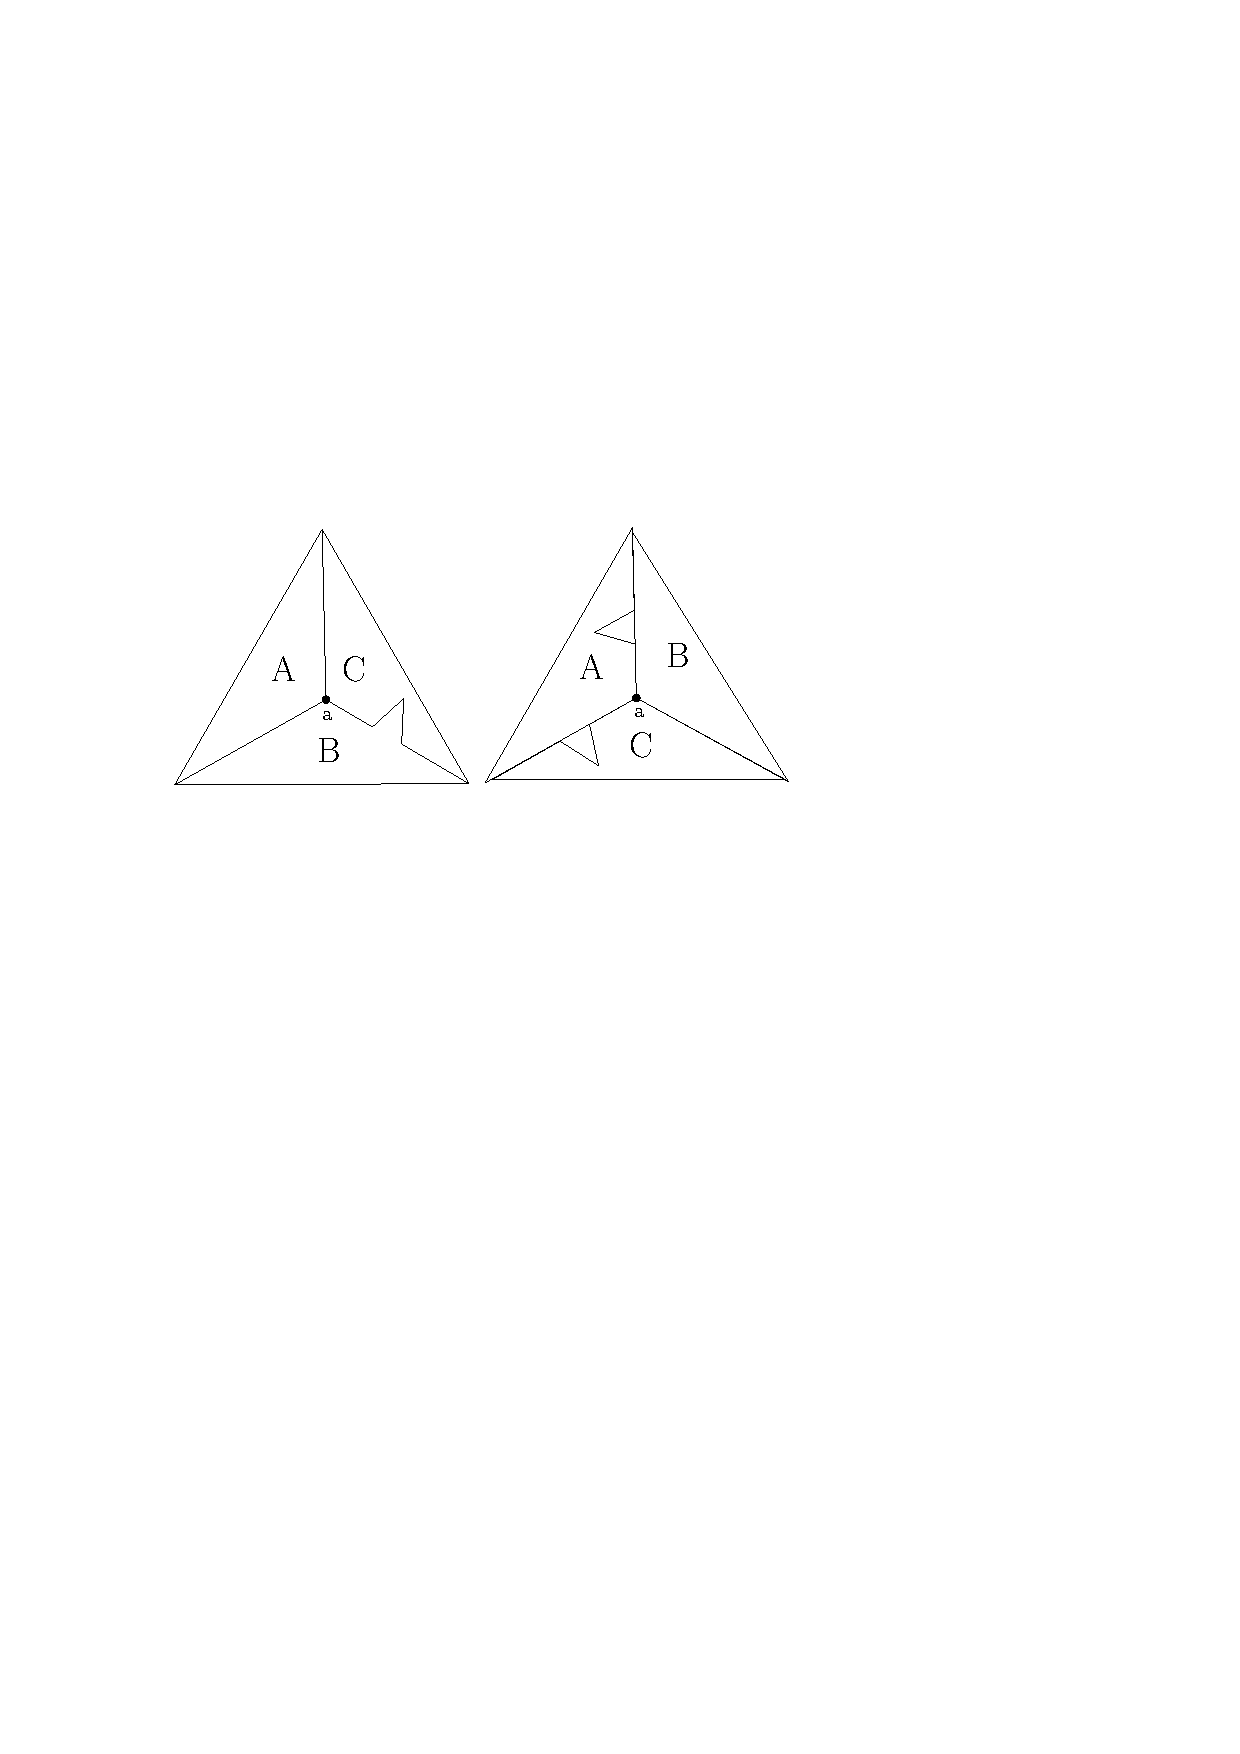
\includegraphics[width=\linewidth]{graphics/orderedFaces.pdf}
		\end{center}
    \end{minipage}
  \end{columns}
\end{frame}

\begin{frame}
\frametitle{Motivation: Weighted Trees and Disk Arrangements}
\begin{prob}
Decide whether a given ordered tree with positive vertex weights is the contact graph of a disk arrangements with specified radii?
\end{prob}
\begin{columns}[c] % the "c" option specifies center vertical alignment
  \column{.5\textwidth} % column designated by a command
   \begin{itemize}
    \item Breu and Kirkpatrick proved that it is NP-Hard to decide whether a graph G is the contact graph of unit disks in the plane, i.e., recognizing coin graphs is NP-Hard
   \end{itemize}
  \column{.5\textwidth}
    \begin{minipage}{\linewidth}
        \begin{center}
        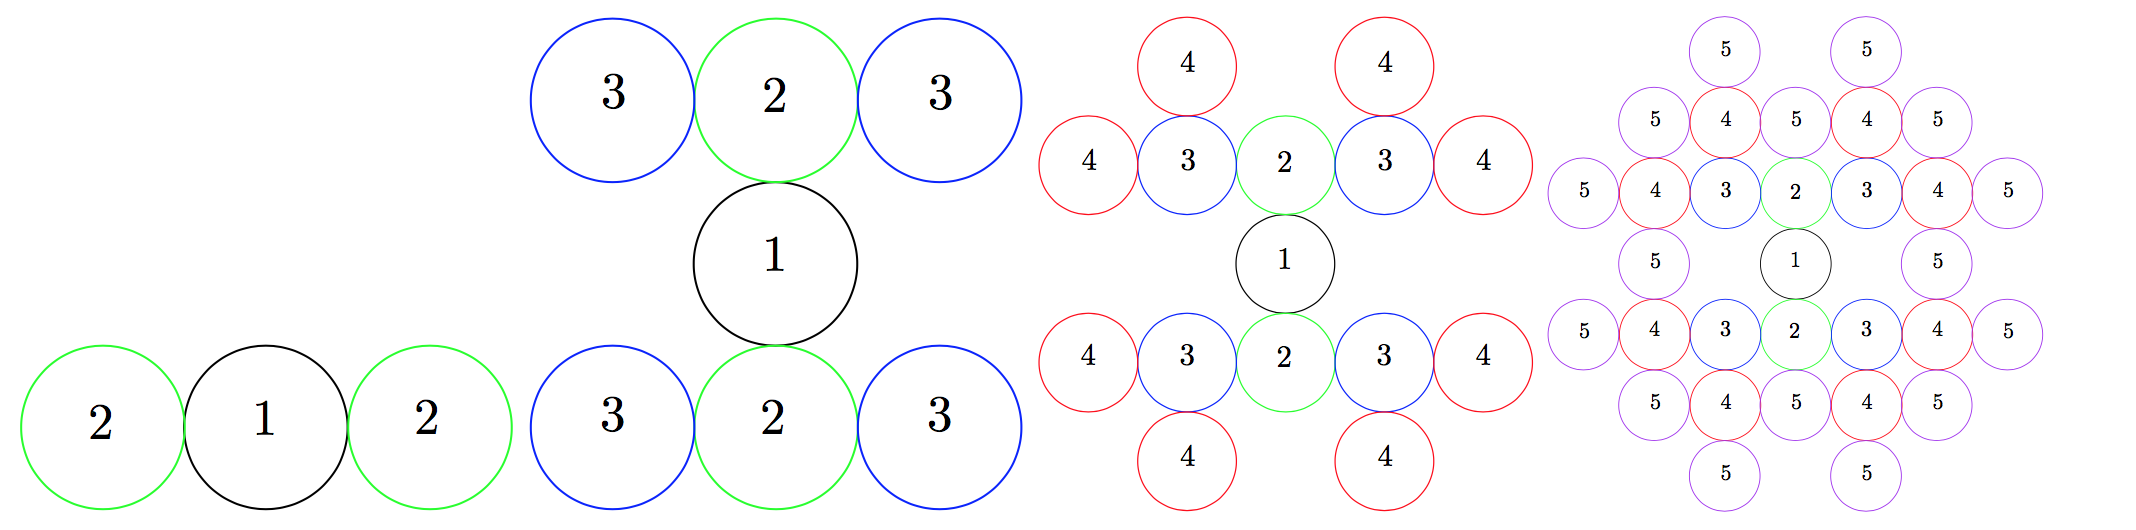
\includegraphics[width=\linewidth]{graphics/diskArrangementExample.png}
        \end{center}
    \end{minipage}
  \end{columns}
\end{frame}

\begin{frame}\frametitle{Problem: Weighted Trees and Disk Arrangements}
    \begin{columns}[c]
    \column{.5\textwidth}
        \begin{itemize}
            \item[*] Is it NP-hard to decide whether a polygonal linkage whose hinge graph is a \textit{tree} can be realized? 
            \item[*] Is it NP-Hard to decide whether a given ordered tree with positive vertex weights is the contact graph of a disk arrangements with specified radii?
        \end{itemize}
    \column{.5\textwidth}
        \begin{minipage}{\linewidth}
            \begin{center}
            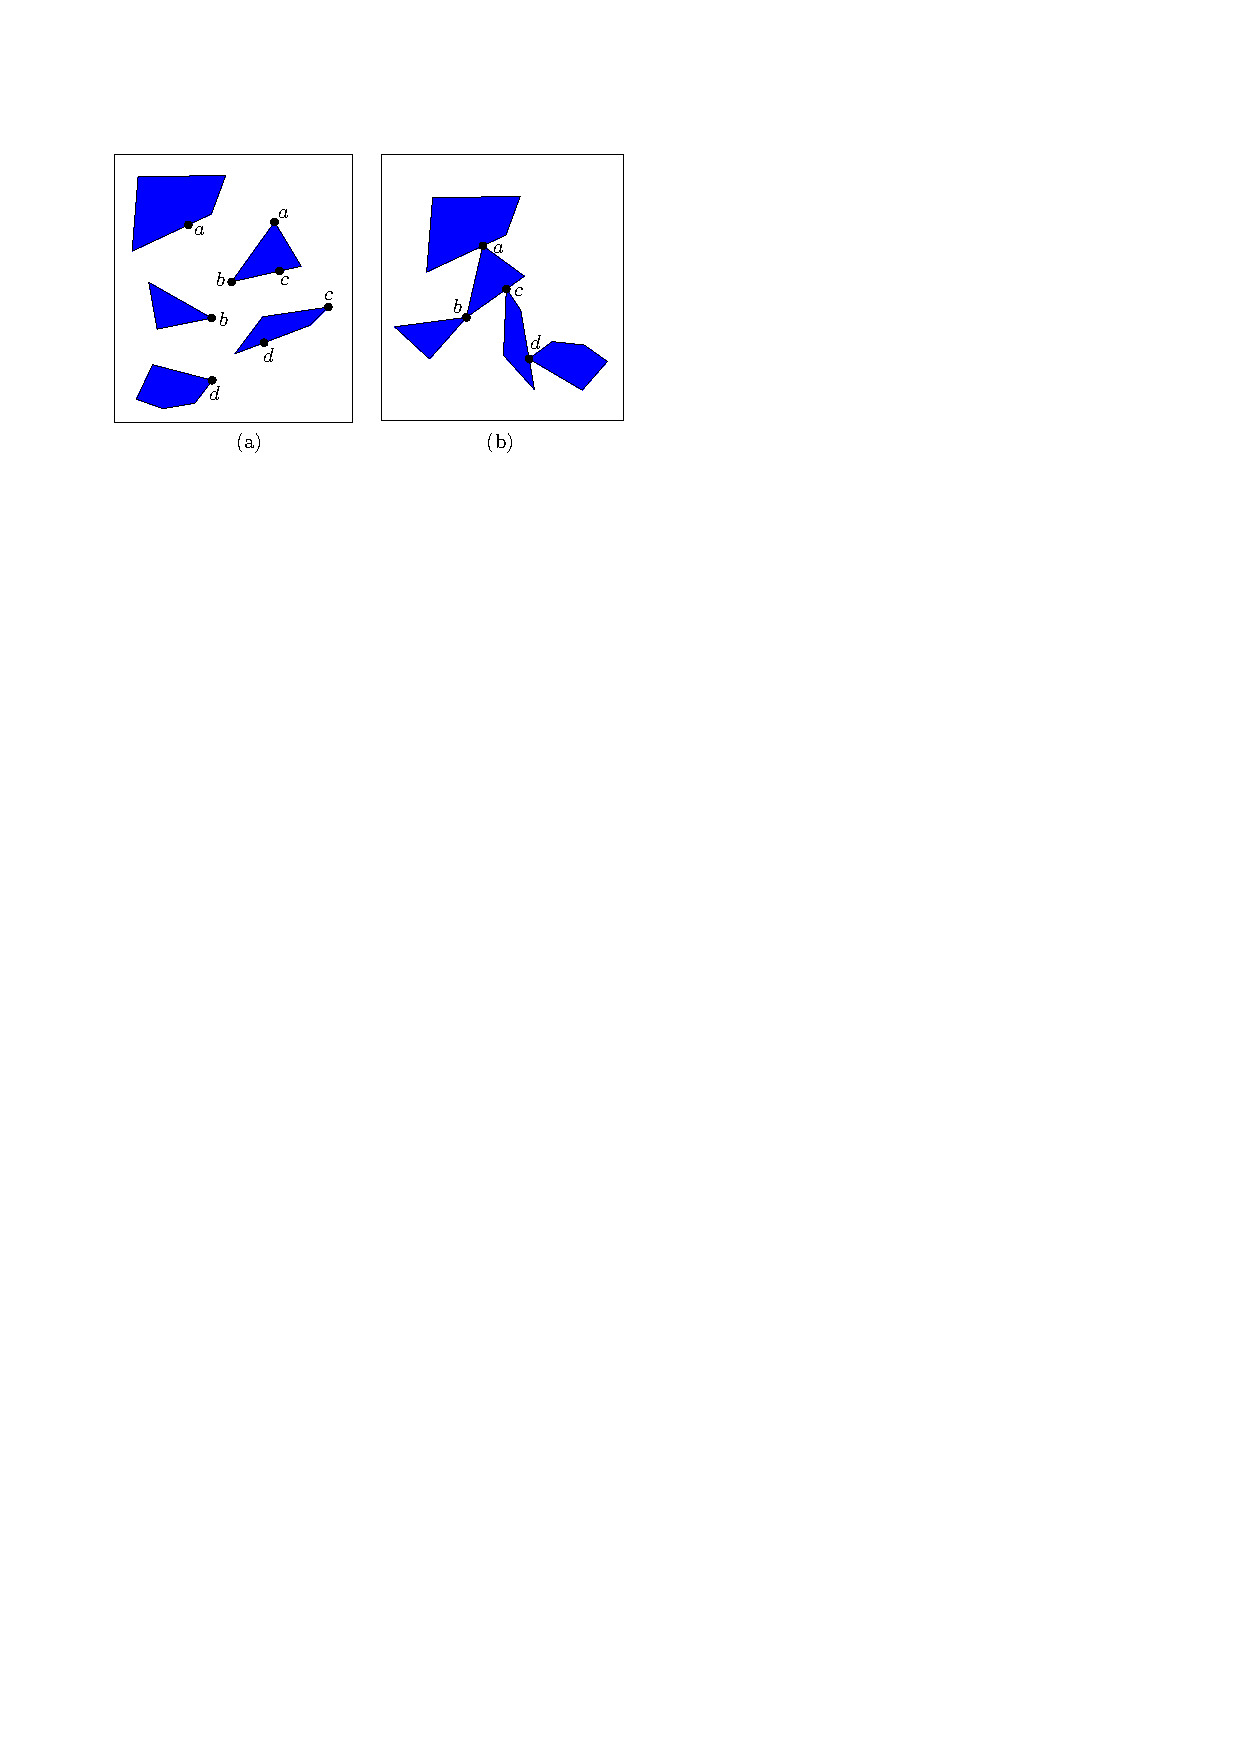
\includegraphics[width=.9\textwidth]{graphics/fig1++.pdf}
            \end{center}
        \end{minipage}
    \end{columns}
\end{frame}

% \begin{frame}\frametitle{Motivation: Weighted Trees and Disk Arrangements}
%     \begin{columns}[c]
%     \column{.5\textwidth}
%         \begin{itemize}
%             \item[*] Is it NP-Hard to decide whether a polygonal linkage whose hinge graph is a \textit{tree} can be realized? 
%             \item[*] Is it NP-Hard to decide whether a given ordered tree with positive vertex weights is the contact graph of a disk arrangements with specified radii?
%         \end{itemize}
%     \column{.5\textwidth}
        
%     \end{columns}
% \end{frame}


\begin{frame} \frametitle{Related Work}

\begin{itemize}
	\item[*] Bhatt and Cosmadakis showed that deciding whether a polygonal linkage whose hinge graph is a \textit{graph} is NP-Hard.
	\item[*] Breu and Kirkpatrick showed that deciding whether a given ordered tree with unit vertex weights is the contact graph of a disk arrangements with specified radii.
\end{itemize}
    % \begin{columns}[c]
    % \column{.5\textwidth}
        
    % \column{.5\textwidth}
    % \begin{minipage}{\linewidth}
    %         \begin{center}
    %         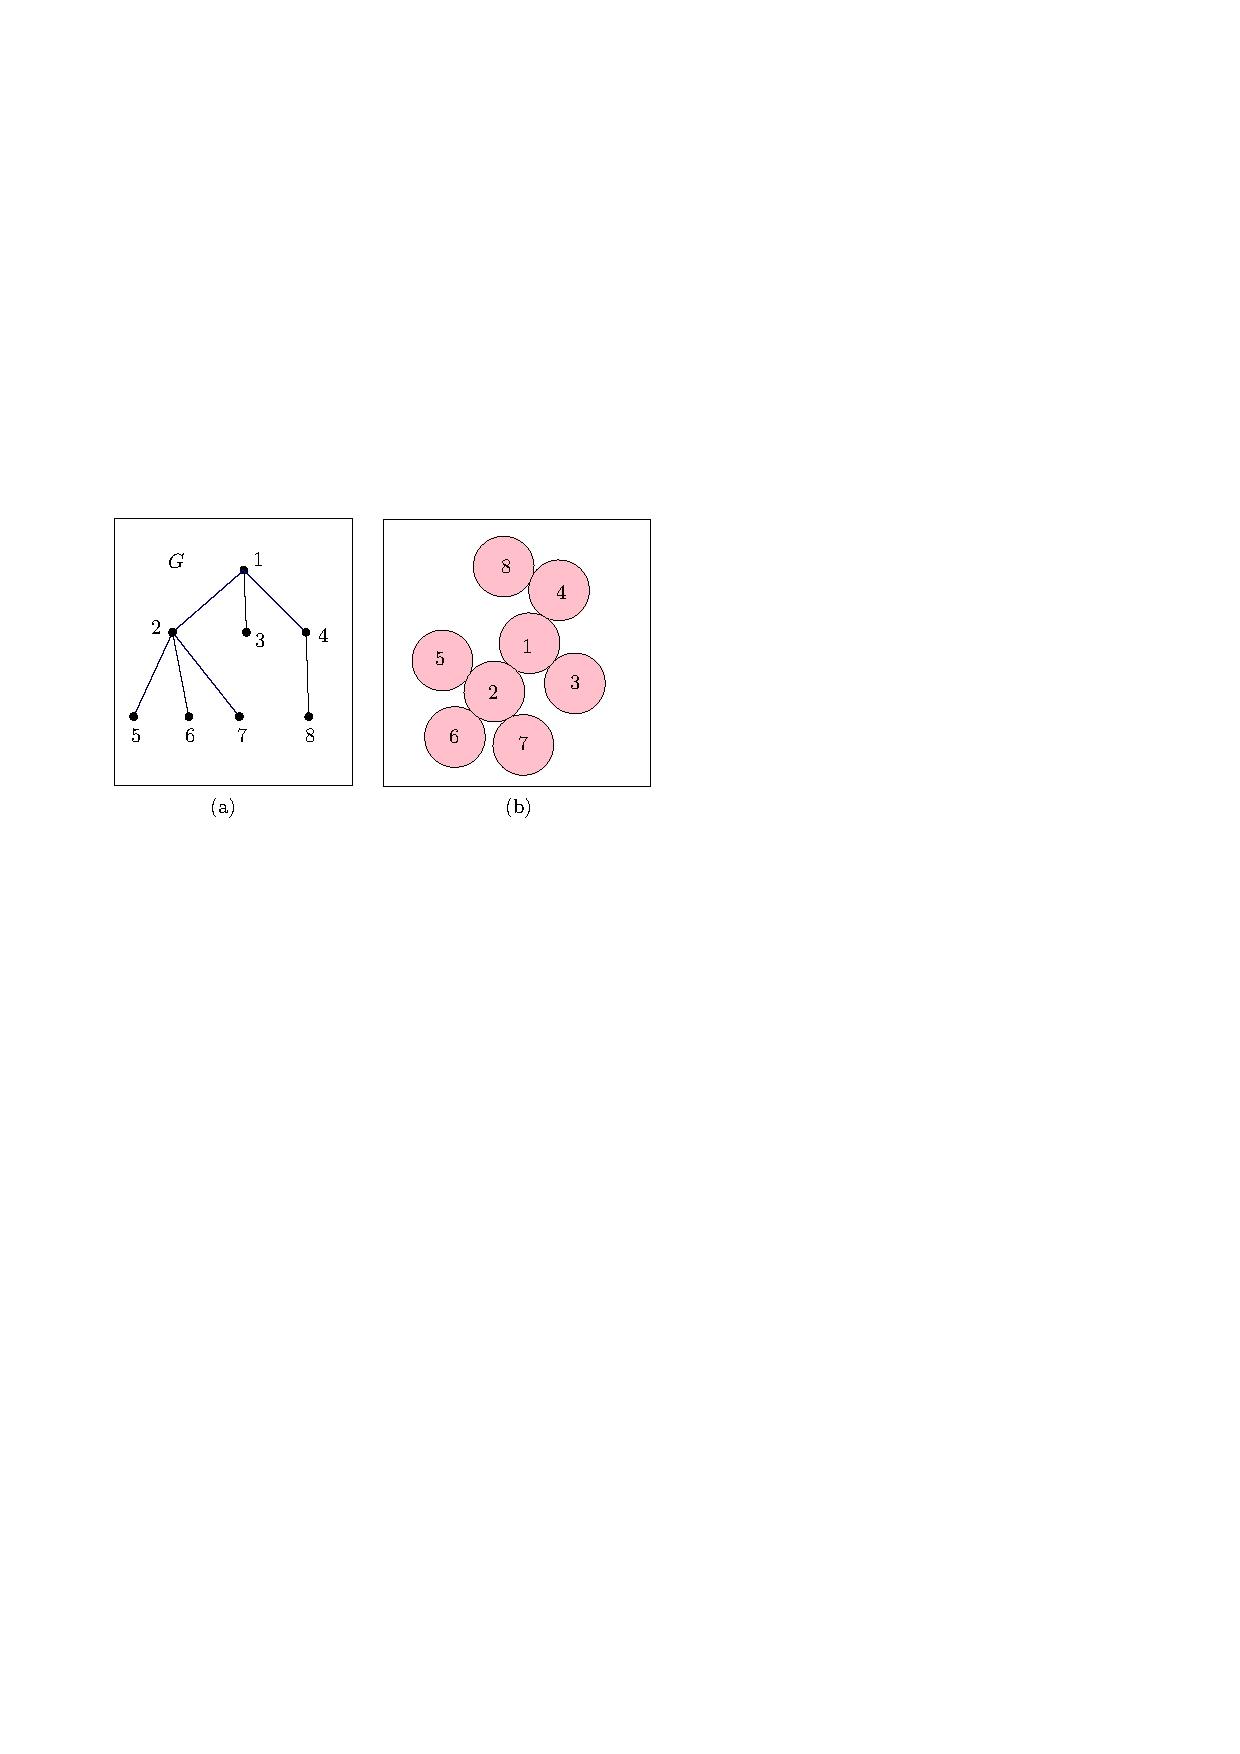
\includegraphics[width=.9\textwidth]{graphics/fig3++.pdf}
    %         \end{center}
    %     \end{minipage}
    % \end{columns}
\end{frame}

\begin{frame}\frametitle{Contributions}
     \begin{thm}
     It is NP-Hard to decide whether a polygonal linkage whose hinge graph is a \textit{tree} can be realized.
     \end{thm}
    \begin{thm} It is NP-Hard to decide whether a polygonal linkage whose hinge graph is a \textit{tree} can be realized with fixed orientation.
    \end{thm}
    \begin{thm} It is NP-Hard to decide whether a given ordered tree with positive vertex weights is the contact graph of a disk arrangements with specified radii.
    \end{thm}
\end{frame}

\begin{frame} \frametitle{The Logic Engine}
    \begin{columns}[c]
    \column{.5\textwidth}
        \begin{minipage}{\linewidth}
            \begin{center}
            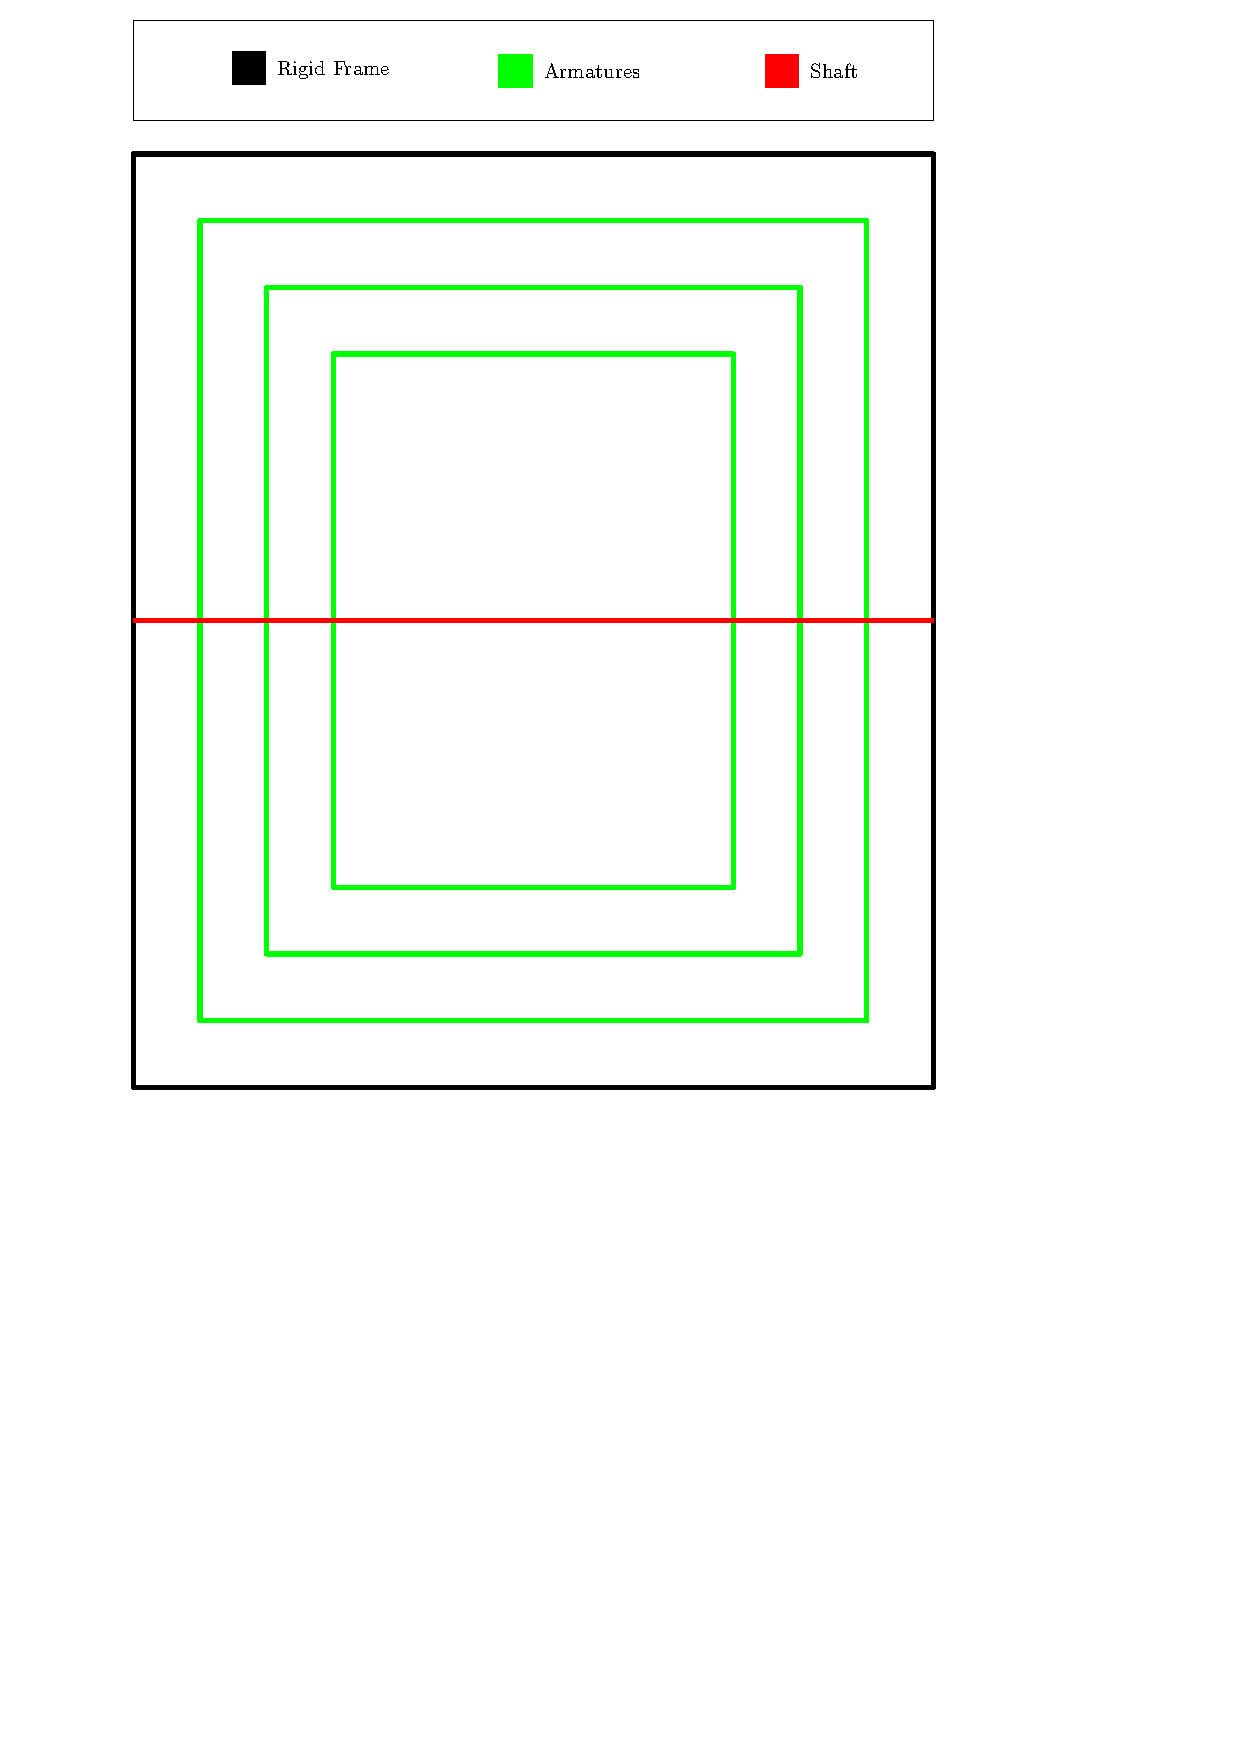
\includegraphics[width=.9\textwidth]{graphics/LogicEngineFrame.pdf}
            \end{center}
        \end{minipage}
    \column{.5\textwidth}
        \begin{minipage}{\linewidth}
            \begin{center}
            \includegraphics[width=.9\textwidth]{graphics/LogicEngineFrameFigure2.pdf}
            \end{center}
        \end{minipage}
    \end{columns}
\end{frame}

\begin{frame} \frametitle{Logic Engine Realized as Hinged Polygons}
    \begin{columns}[c]
    \column{.5\textwidth}
        \begin{itemize}
            \item[*] Suppose we are given an Boolean formula with $m$ clauses and $n$ variables in 3-CNF form, $\Phi$, we construct the polygonal linkage similarly to the logic engine.
        \end{itemize}
    \column{.5\textwidth}
        \begin{minipage}{\linewidth}
            \begin{center}
            \includegraphics[width=.9\textwidth]{graphics/HingedLogicEngineSmallEnumerated.pdf}
            \end{center}
        \end{minipage}
    \end{columns}
\end{frame}

% \begin{frame} \frametitle{Logic Engine Realized as Hinged Polygons}
%     \begin{columns}[c]
%     \column{.5\textwidth}
%         \begin{itemize}
%             % \item[*] Breu and Kirkpatrick~\cite{BK98} proved that it is NP-hard to decide whether a graph $G$ is the contact graph of unit disks in the plane, i.e., recognizing \emph{coin graphs} is NP-hard; see also~\cite{BET+99}.
%             \item here
%         \end{itemize}
%     \column{.5\textwidth}
%     \begin{itemize}
%             % \item[*] Bhatt and Cosmadakis~\cite{BC87}, who proved that the realizability of linkages is NP-complete on the integer grid.
%             \item three
%         \end{itemize}
%     \end{columns}
% \end{frame}

\begin{frame} \frametitle{Planar 3SAT}
    \begin{columns}[c]
    \column{.5\textwidth}
        \begin{itemize}
            \item[*] Given a Boolean formula $\Phi$ in 3-CNF such that the associated graph is $A(\Phi)$, decide whether it 
is satisfiable is the \textit{3-SAT problem}.
        \end{itemize}
    \column{.5\textwidth}
        \begin{minipage}{\linewidth}
            \begin{center}
            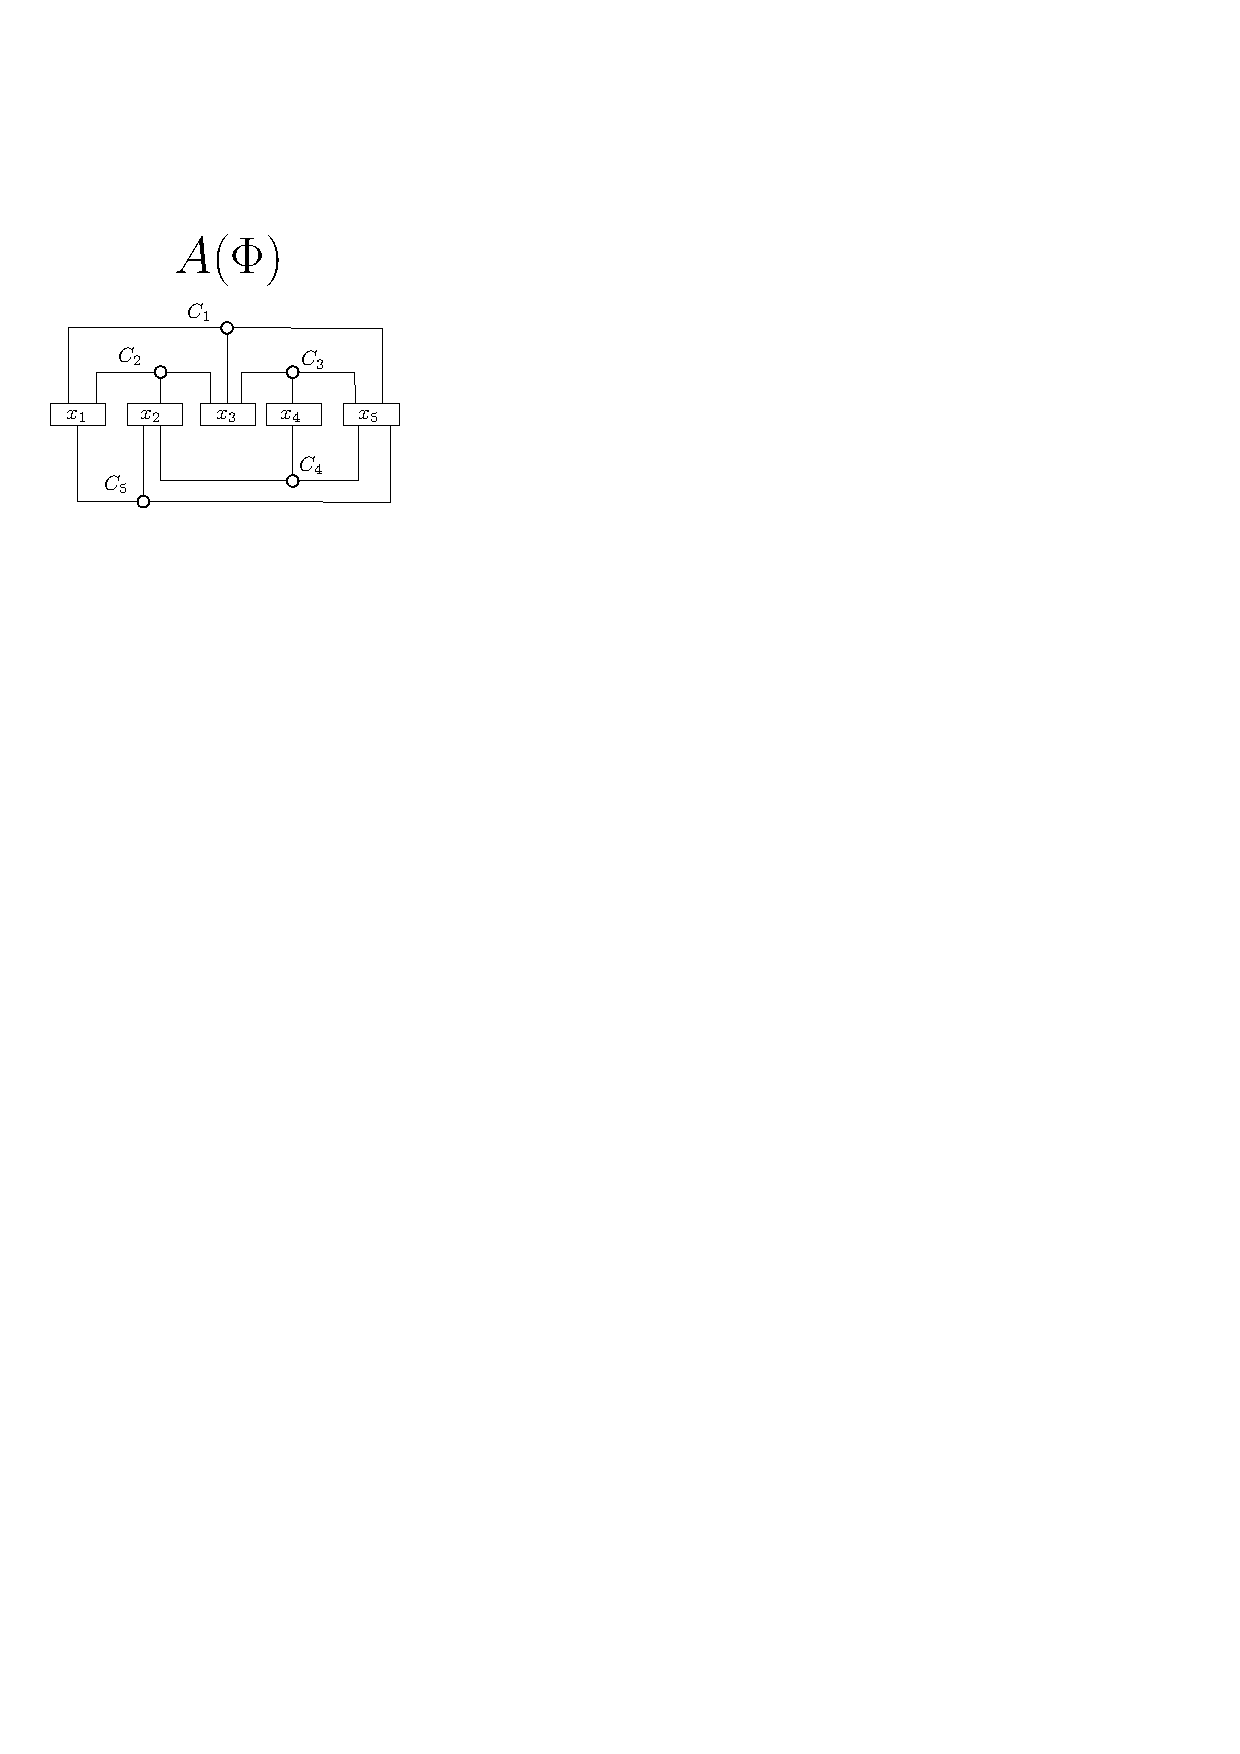
\includegraphics[width=.9\textwidth]{graphics/fig-assoc-hex2.pdf}
            \end{center}
        \end{minipage}
    \end{columns}
\end{frame}
\begin{frame} \frametitle{Modified Auxiliary Construction}
    \begin{columns}[c]
    \column{.5\textwidth}
        \begin{itemize}
            \item[*] Define the \textit{associated graph} $A(\Phi)$ as follows: the vertices correspond to the variables and clauses in $\Phi$.   
We place an edge in the graph if variable $x_i$ appears in clause $C_j$.
            \item[*] Given a Boolean formula $\Phi$ in 3-CNF such that its associated graph is planar, decide whether it 
is satisfiable is a \textit{3-SAT problem}.
        \end{itemize}
    \column{.5\textwidth}
        \begin{minipage}{\linewidth}
            \begin{center}
            \includegraphics[width=.66\textwidth]{graphics/honeycomb.pdf}
            % 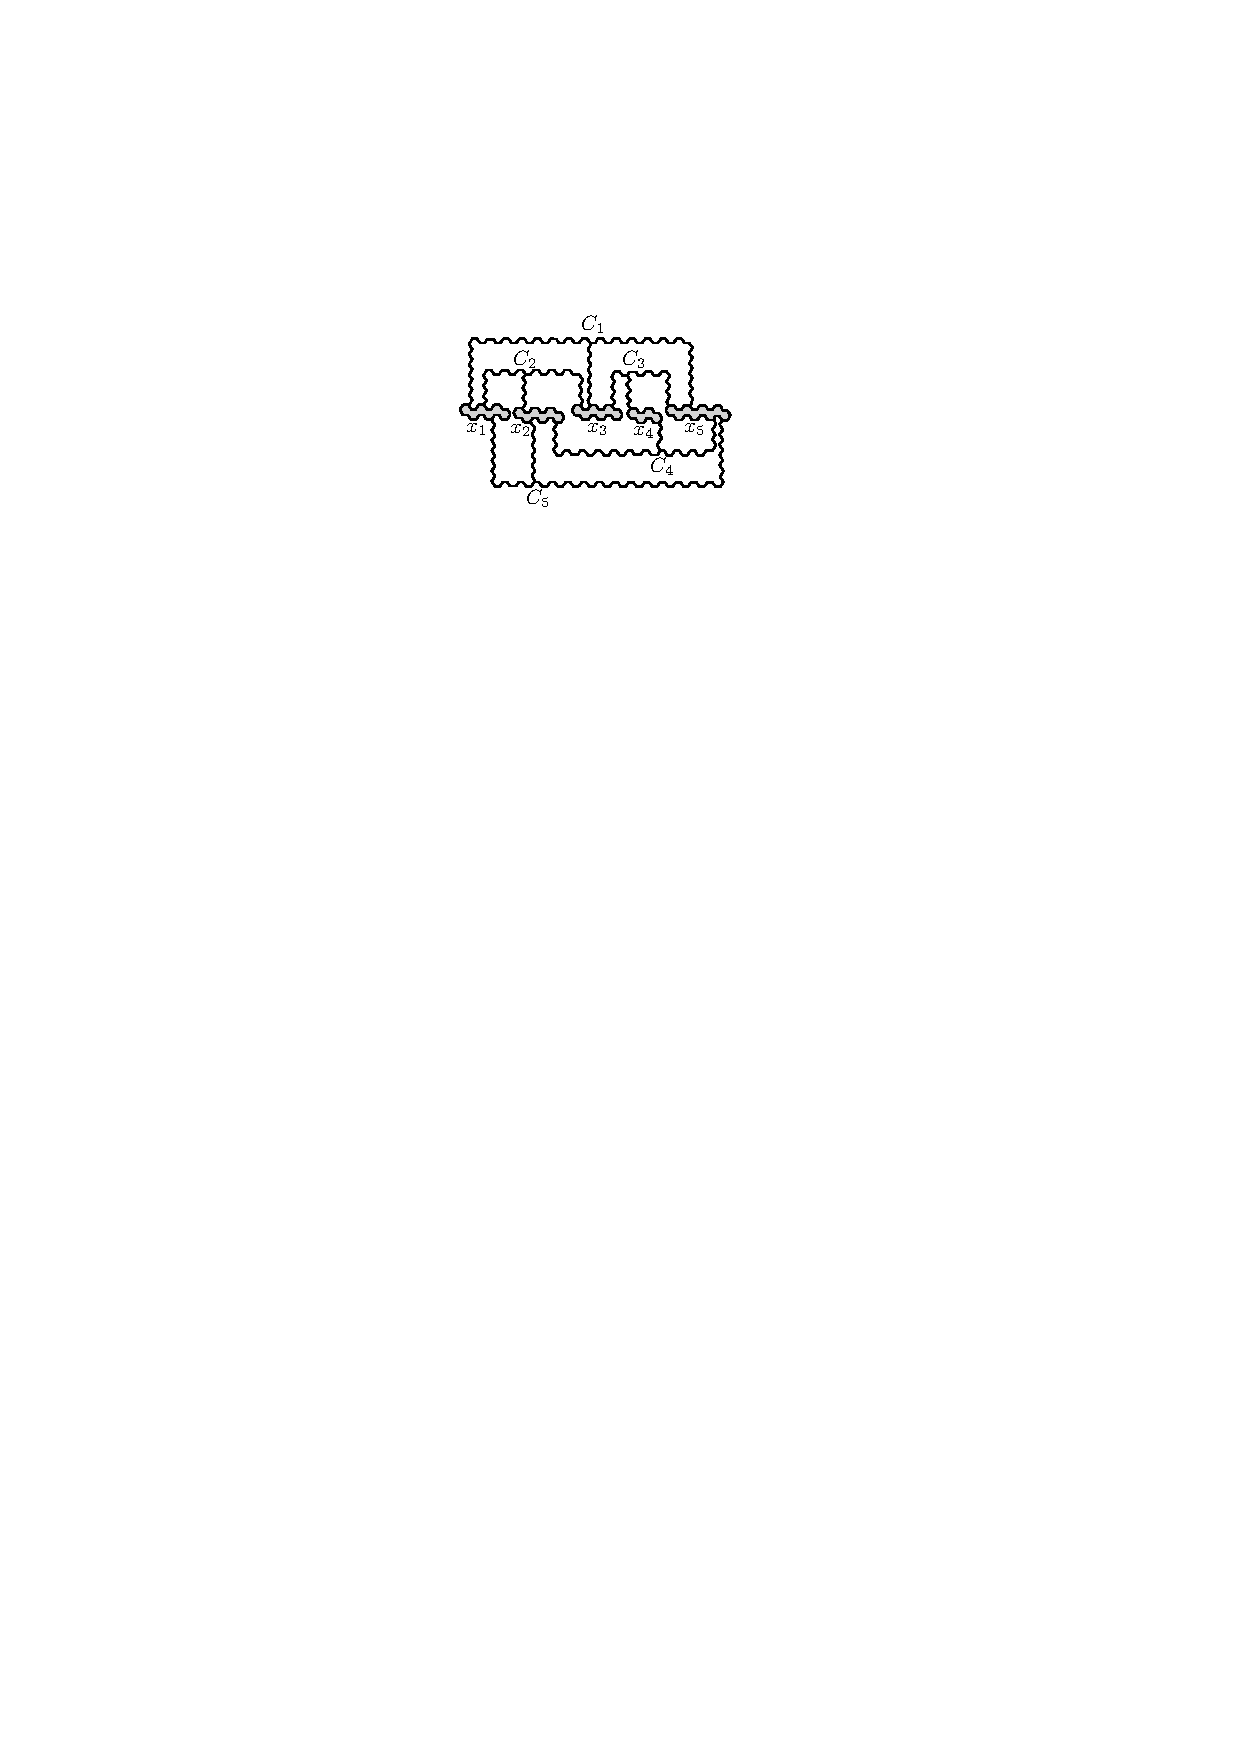
\includegraphics[width=.66\textwidth]{graphics/fig-assoc-hex1.pdf}
            \end{center}
        \end{minipage}
    \end{columns}
\end{frame}
\begin{frame} \frametitle{Modified Auxiliary Construction}
    \begin{columns}[c]
    \column{.5\textwidth}
        \begin{itemize}
            \item[*] Define the \textit{associated graph} $A(\Phi)$ as follows: the vertices correspond to the variables and clauses in $\Phi$.   
We place an edge in the graph if variable $x_i$ appears in clause $C_j$.
            \item[*] Given a Boolean formula $\Phi$ in 3-CNF such that its associated graph is planar, decide whether it 
is satisfiable is a \textit{3-SAT problem}.
        \end{itemize}
    \column{.5\textwidth}
        \begin{minipage}{\linewidth}
            \begin{center}
            % \includegraphics[width=.66\textwidth]{graphics/honeycomb.pdf}
            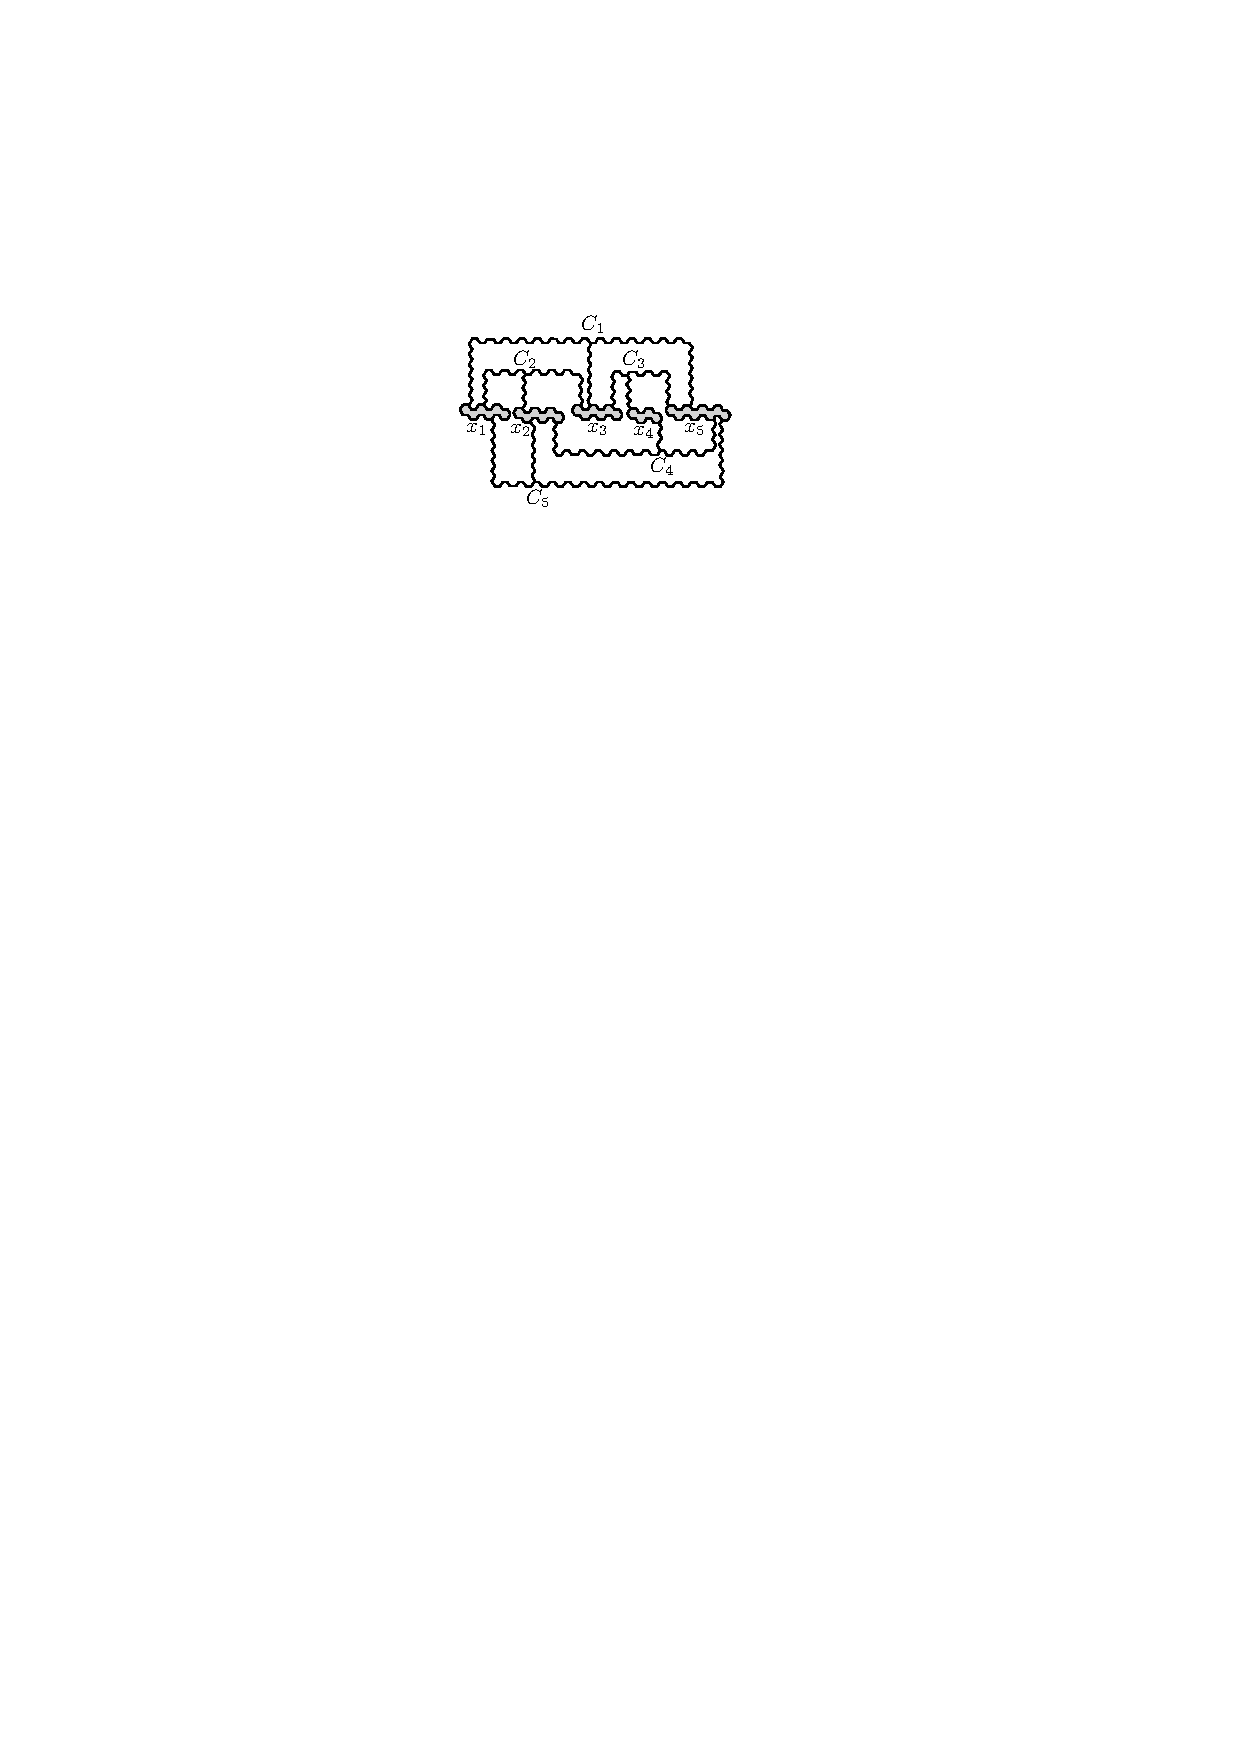
\includegraphics[width=.66\textwidth]{graphics/fig-assoc-hex1.pdf}
            \end{center}
        \end{minipage}
    \end{columns}
\end{frame}

\begin{frame} \frametitle{Transmitter Gadget}
    \begin{columns}[c]
    \column{.5\textwidth}
        \begin{itemize}
            \item[*] A {\it transmitter gadget} is constructed for each edge $\left\lbrace x_i,C_j\right\rbrace$ of the graph $A(\Phi)$; it consists of a sequence of junctions and corridors from a variable gadget's junction to a clause junction.  
        \end{itemize}
    \column{.5\textwidth}
        \begin{minipage}{\linewidth}
            \begin{center}
            \includegraphics[width=.75\textwidth]{graphics/FalseVariableNonNegatedLiteralTransmitter-Beamer.pdf}
            \end{center}
        \end{minipage}

        \begin{minipage}{\linewidth}
            \begin{center}
            \includegraphics[width=.9\textwidth]{graphics/VariableGadgetTruthness.pdf}
        \end{center}
        \end{minipage}
    \end{columns}
\end{frame}

\begin{frame} \frametitle{Variable Gadget}
    \begin{columns}[c]
    \column{.5\textwidth}
        \begin{itemize}
            \item[*] Variable $x_i$ corresponds to a cycle in the associated graph $\tilde{A}(\Phi)$. 
        \end{itemize}
    \column{.5\textwidth}
                    \begin{minipage}{\linewidth}
            \begin{center}
            \includegraphics[width=.9\textwidth]{graphics/VariableGadgetSmall-Beamer.pdf}
            \end{center}
        \end{minipage}
    \end{columns}
\end{frame}

\begin{frame} \frametitle{Variable Gadget}
    \begin{columns}[c]
    \column{.5\textwidth}
        \begin{itemize}
            \item[*] Variable $x_i$ corresponds to a cycle in the associated graph $\tilde{A}(\Phi)$. 
        \end{itemize}
    \column{.5\textwidth}
                    \begin{minipage}{\linewidth}
            \begin{center}
            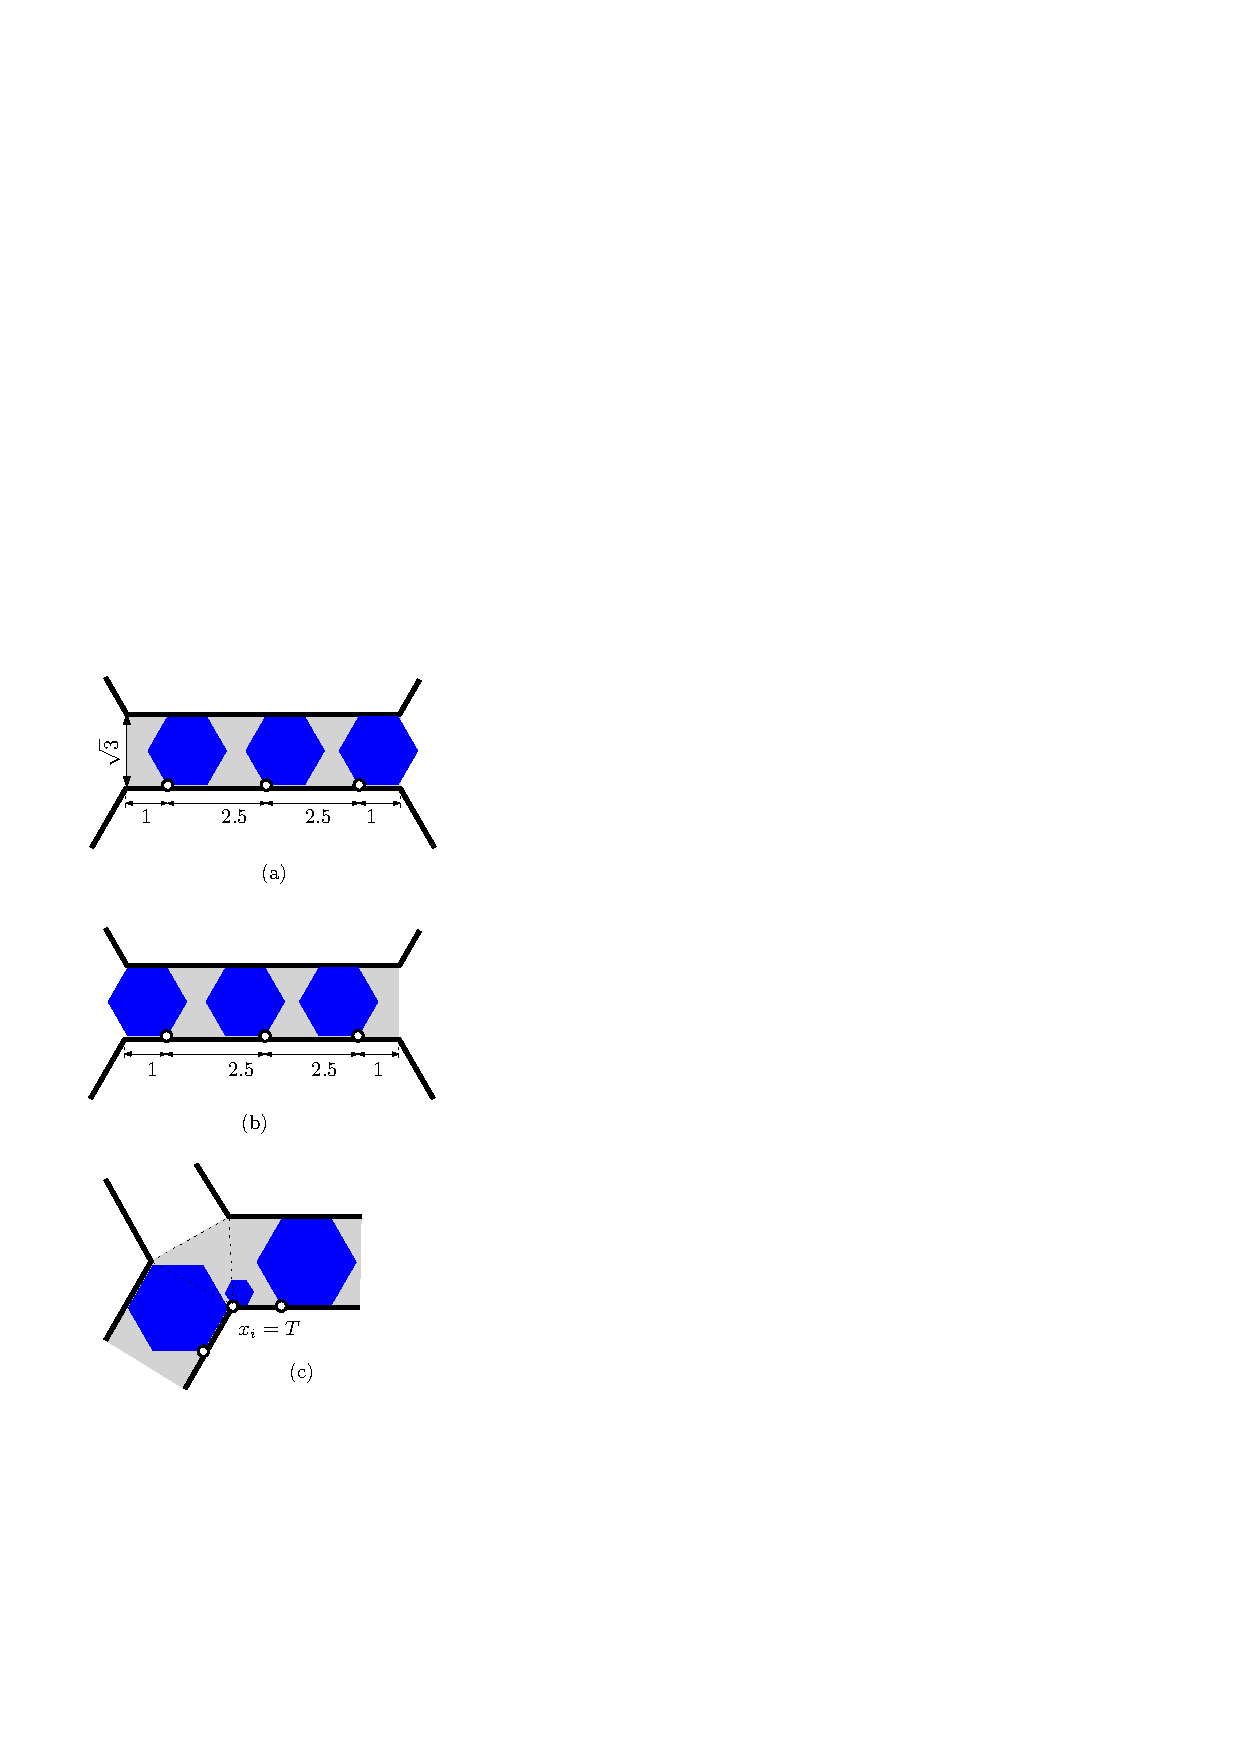
\includegraphics[width=.6\textwidth]{graphics/fig-variable-hex++.pdf}
            \end{center}
        \end{minipage}
    \end{columns}
\end{frame}

\begin{frame} \frametitle{Clause Junction Gadget}
    \begin{columns}[c]
    \column{.5\textwidth}
        \begin{itemize}
            \item[*] The {\it clause gadget} lies at a junction adjacent to three transmitter gadgets.x
        \end{itemize}
    \column{.5\textwidth}
        \begin{minipage}{\linewidth}
            \begin{center}
            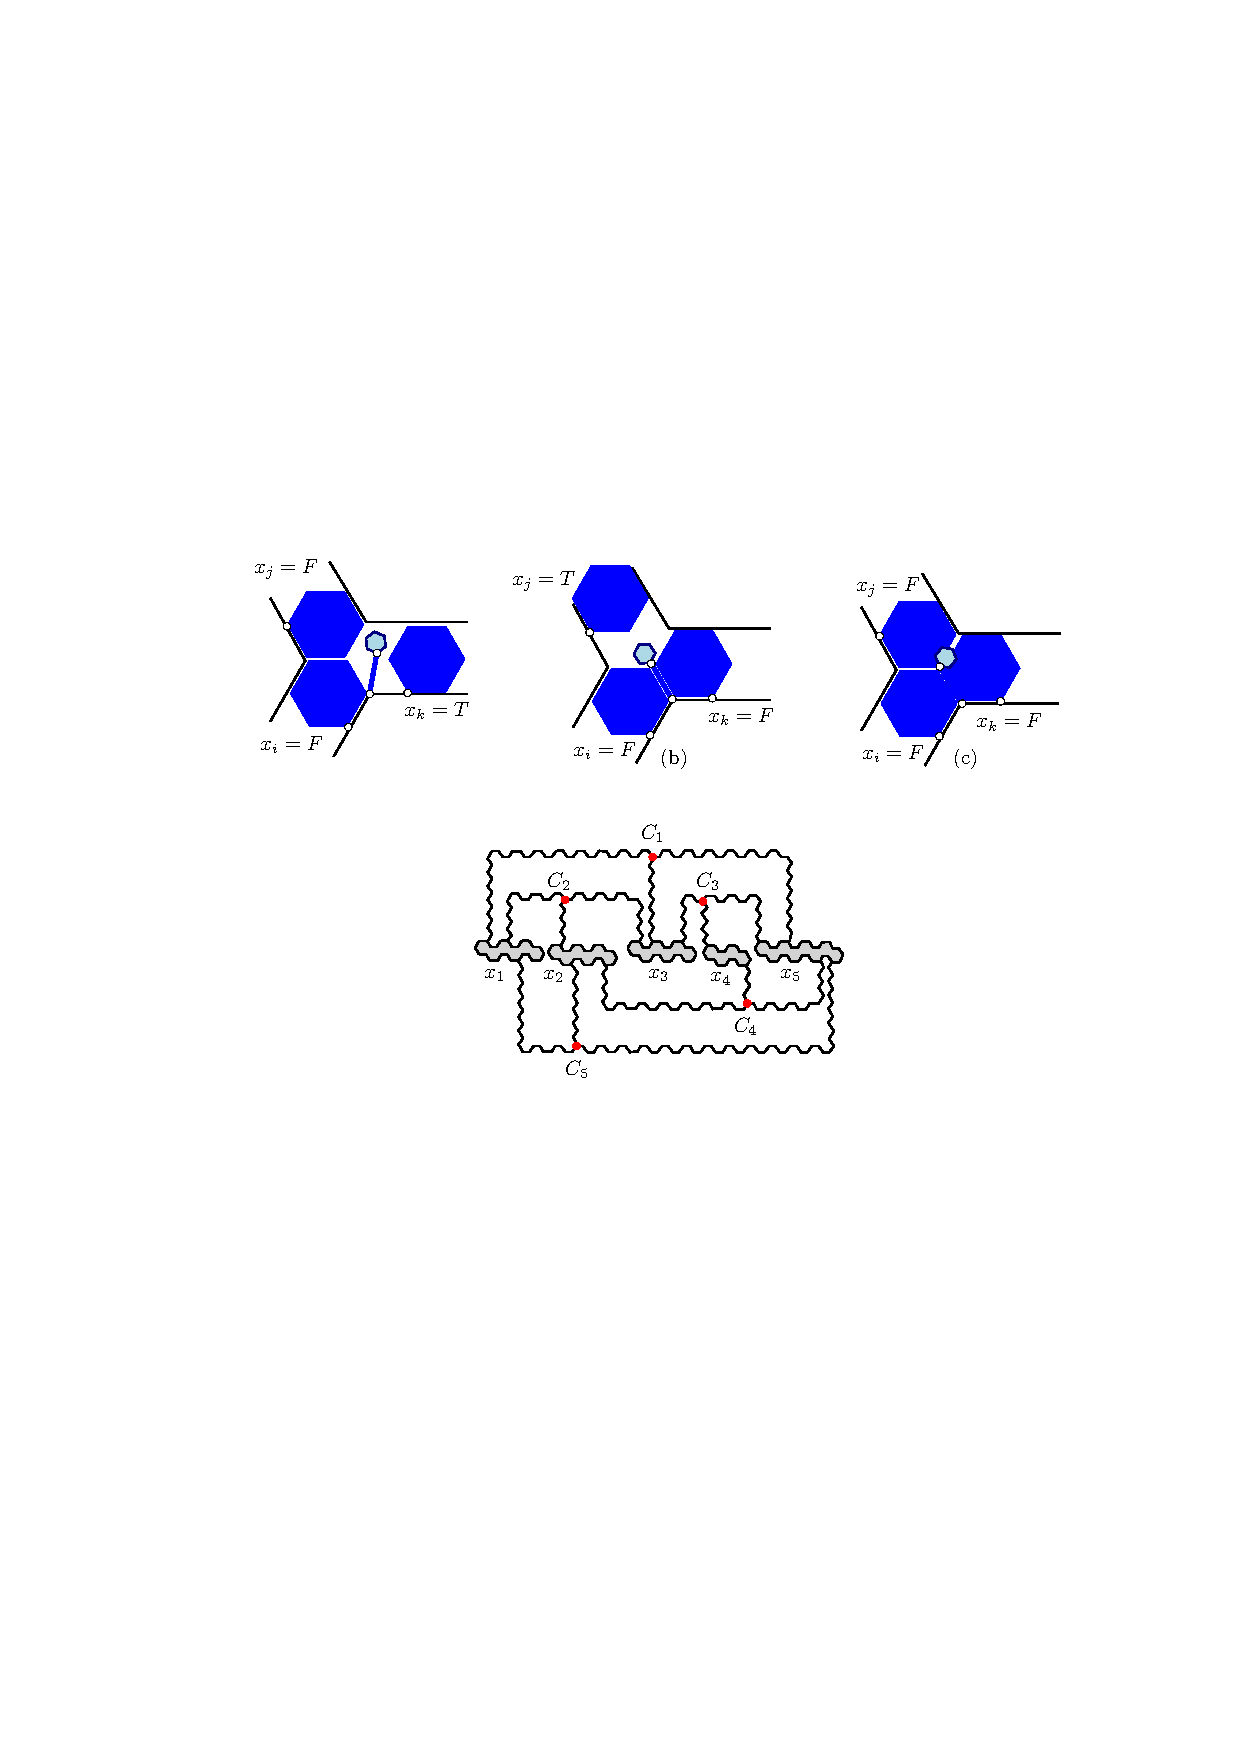
\includegraphics[width=.9\textwidth]{graphics/fig-clause-hex-Beamer.pdf}\label{gfx:fig-clause-hex-Beamer.pdf}
            \end{center}
        \end{minipage}
    \end{columns}
\end{frame}

\begin{frame} \frametitle{Modified Auxiliary Gadget}
    \begin{columns}[c]
    \column{.5\textwidth}
        \begin{itemize}
            \item[*] The modified auxiliary gadget channels and junctions in a hexagonal grid enclosed by six frame hexagons.
        \end{itemize}
    \column{.5\textwidth}
        \begin{minipage}{\linewidth}
            \begin{center}
            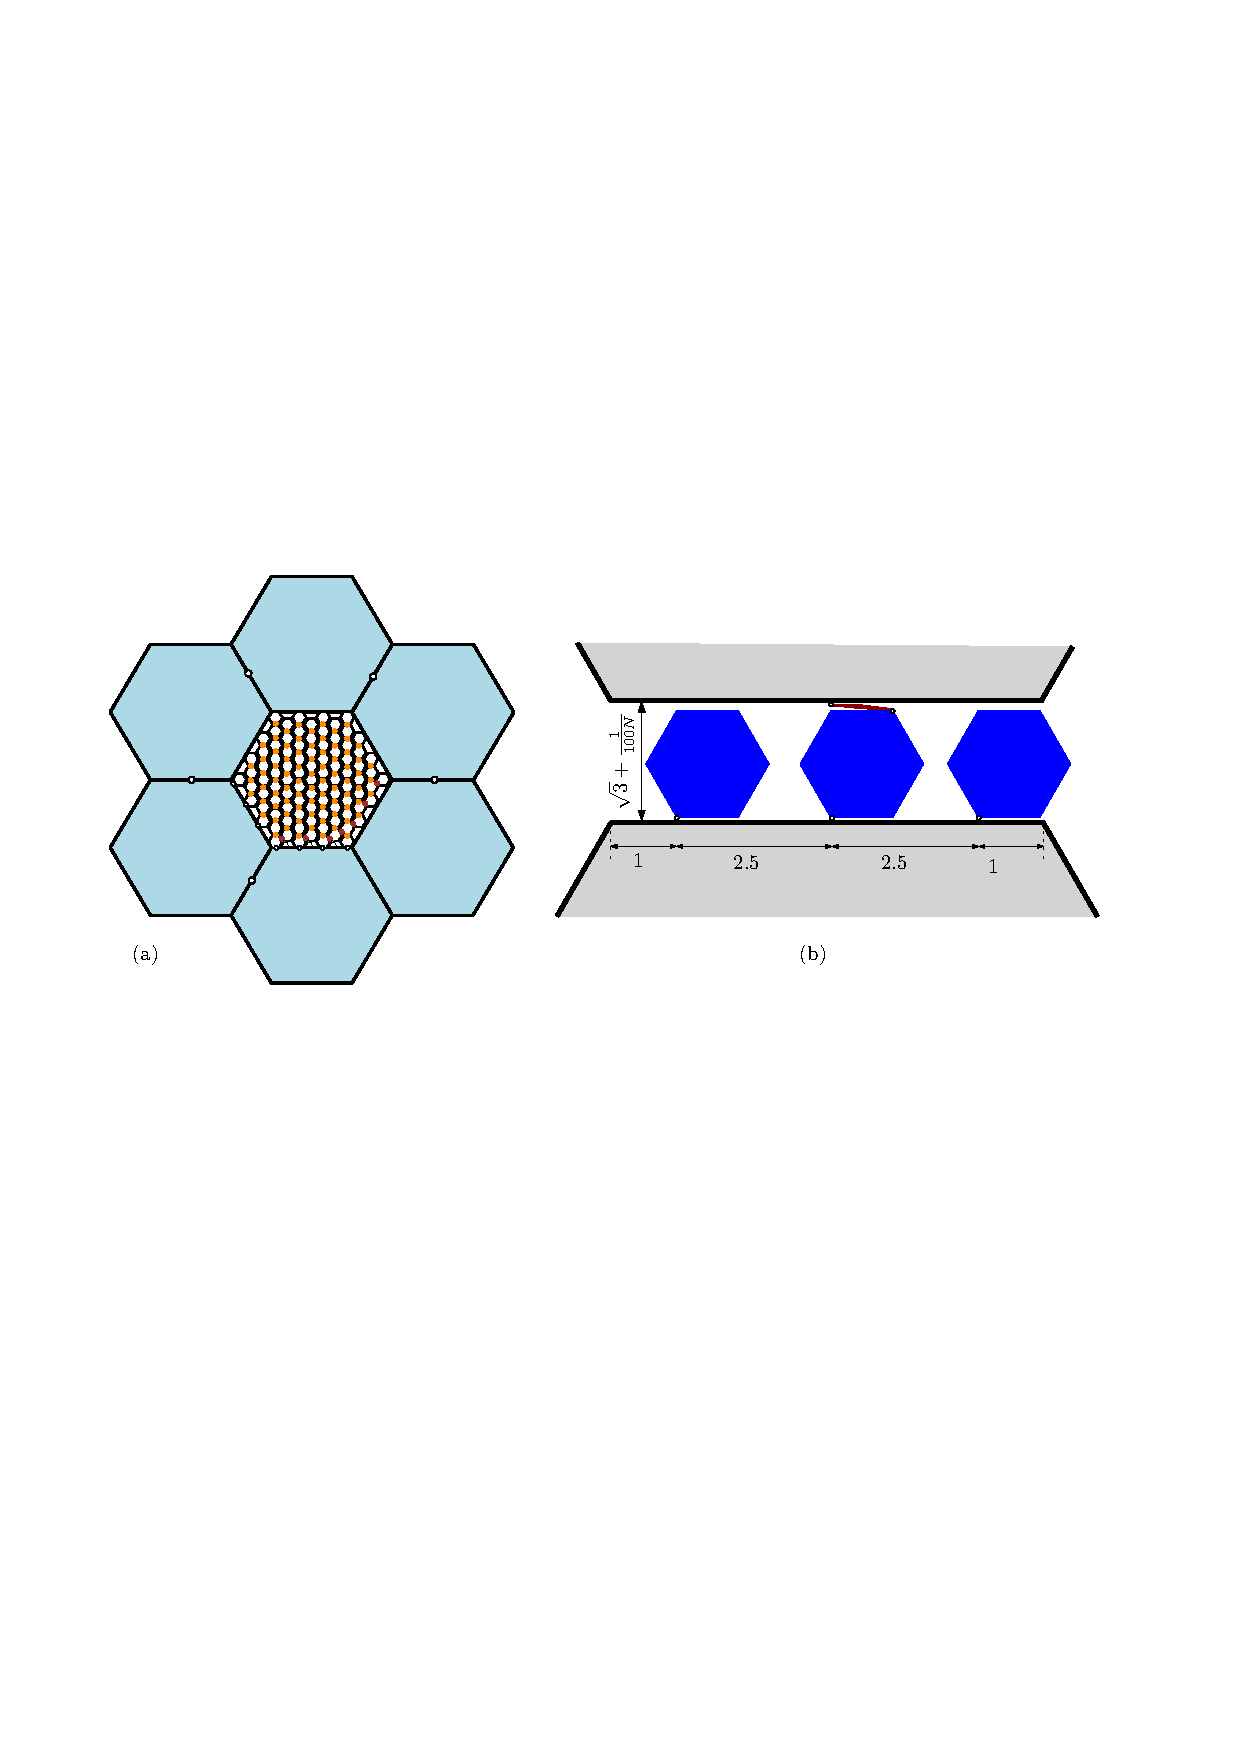
\includegraphics[width=.9\textwidth]{graphics/fig-frame-hex.pdf}\label{gfx:fig-frame-hex.pdf}
            \end{center}
        \end{minipage}
    \end{columns}
\end{frame}
\begin{frame} \frametitle{Approximation of Hexagon with a Disk Arrangement: Hausdorff Distance}
    \begin{columns}[c]
    \column{.5\textwidth}
            \begin{itemize}
            \item[*] An illustrative example of $d(X,Y)$ and $d(Y,X)$ where $X$ is the inner curve, and $Y$ is the outer curve.
            \end{itemize}  
    \column{.5 \textwidth}
        \begin{minipage}{\linewidth}
        \begin{center}
        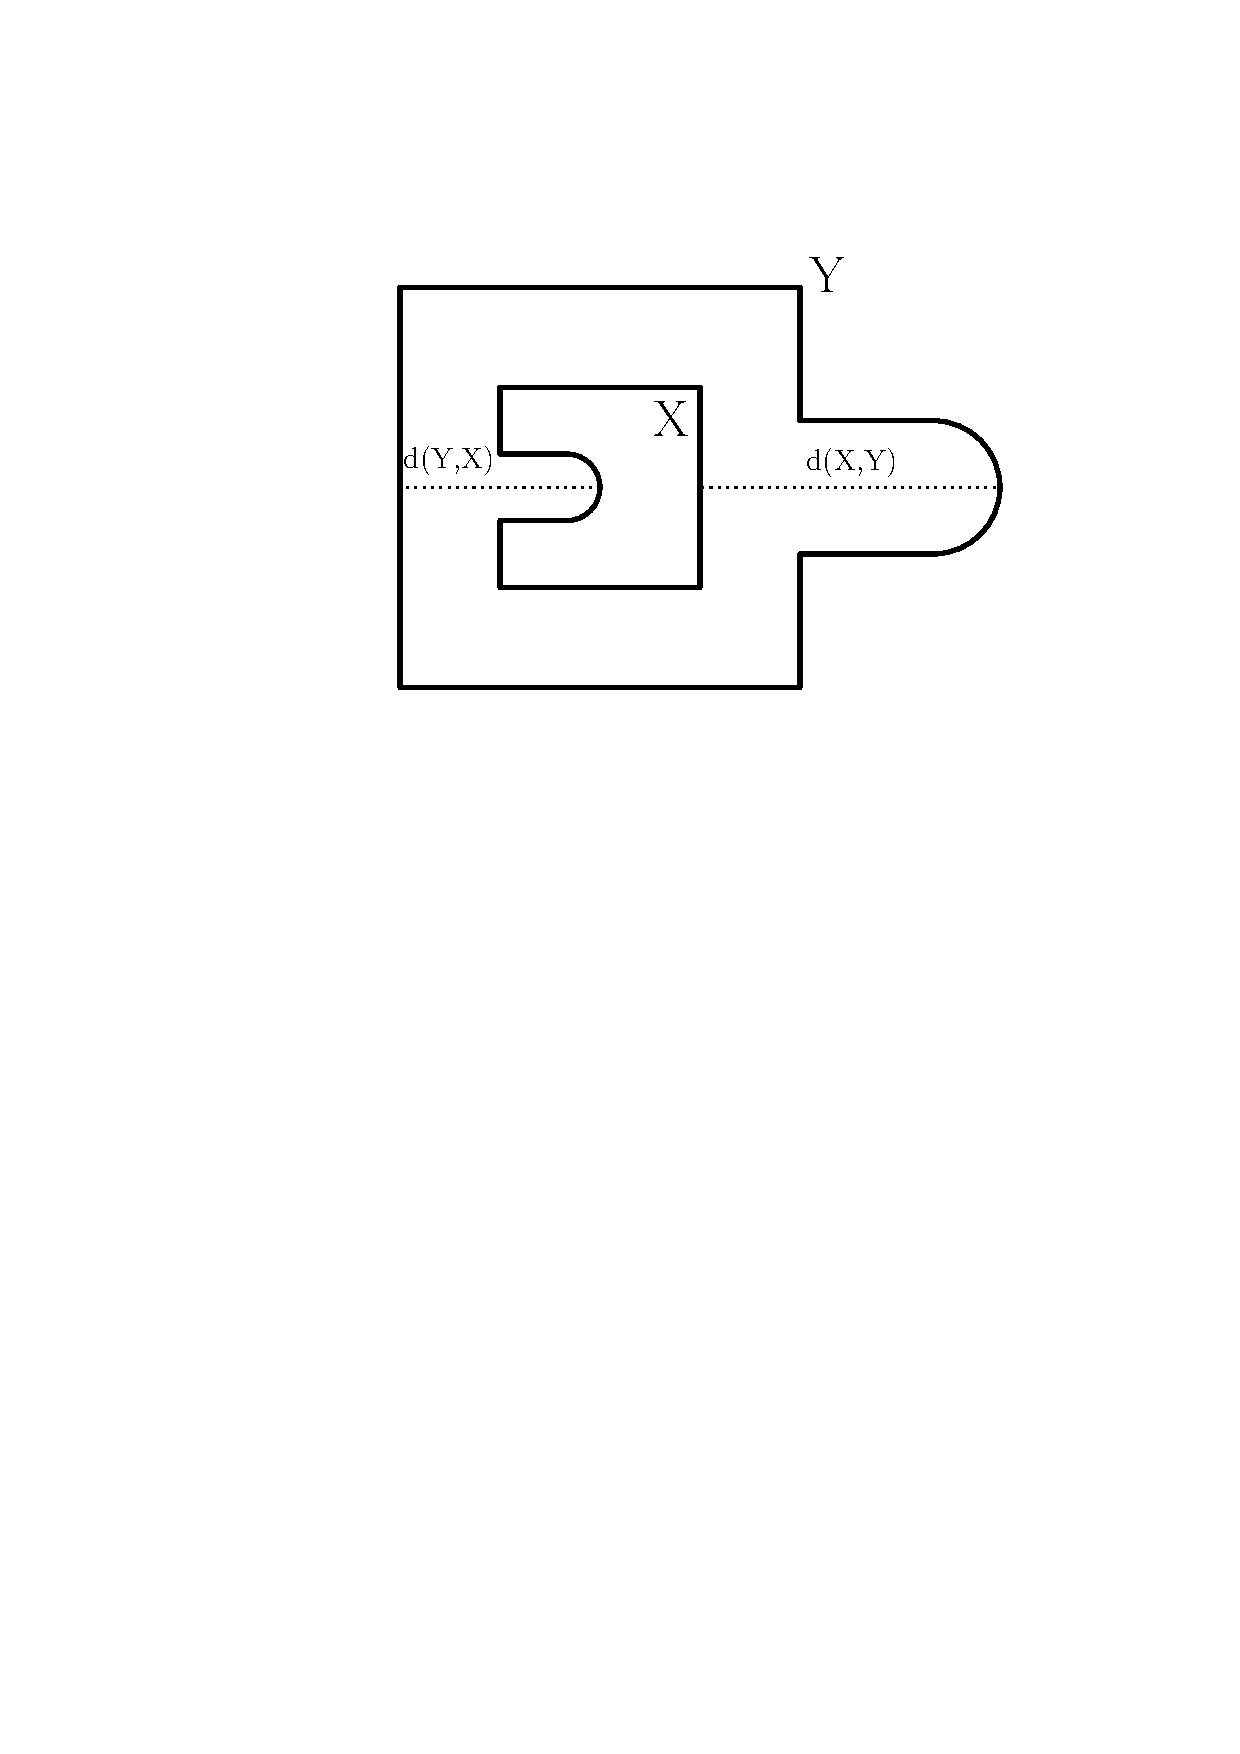
\includegraphics[width=.9\columnwidth]{graphics/HausdorffDistanceExample1.pdf}
        \end{center}
        \end{minipage}
    \end{columns}
\end{frame}

\begin{frame} \frametitle{Approximation of Hexagon with a Disk Arrangement}
    \begin{columns}[c]
    \column{.6\textwidth}
        \begin{lem}
            For every $\epsilon > 0$ and $x>0$, there exists an ordered weighted tree $T$ and regular hexagon $h$ of side length $x$ such that:
            \begin{itemize}
            \item[*] $T$ is realizable.  Every realization $\sigma_i$ of $T$ as an ordered disk contact graph where the radii of the disks equal the vertex weights, approximates the hexagon in the sense that:
            $$H\lr{h,\sigma}\leq\epsilon$$
            \item[*] The number of nodes in $T$ and the weights are polynomial in $\epsilon$ and $x$, the weights $\frac{\epsilon}{10}$ and $\frac{\epsilon}{10} + \zeta$ are polynomial.
            \end{itemize}
        \end{lem}   
    \column{.4\textwidth}
        \begin{minipage}{\linewidth}
            \begin{center}
            \includegraphics[width=.66\textwidth]{graphics/hexagonPetiolesLeafs9Layers.pdf}
            \end{center}
        \end{minipage}
    \end{columns}
\end{frame}

\begin{frame} \frametitle{Approximation of Hexagon with a Disk Arrangement}
    \begin{columns}[c]
    \column{.5\textwidth}
        \begin{itemize}
            \item[*] A drawing of a tree $T$ overlayed with a corresponding disk arrangement, each disk with unit radius.
            \item[*] The nodes of the tree are the centers of the disks.
        \end{itemize}
    \column{.5\textwidth}
        \begin{minipage}{\linewidth}
            \begin{center}
            \includegraphics[width=.9\textwidth]{graphics/hexagonPetiolesLeafs9Layers.pdf}\label{gfx:hexagonPetiolesLeafs9Layers.pdf}
            \end{center}
        \end{minipage}
    \end{columns}
\end{frame}
\begin{frame}\frametitle{Conclusion}
\begin{thm}
     It is strongly NP-Hard to decide whether a polygonal linkage whose hinge graph is a \textit{tree} can be realized.
     \end{thm}
    \begin{thm}It is strongly NP-Hard to diskecide whether a polygonal linkage whose inge graph is a \textit{tree} can be realized with fixed orientation.\end{thm}
    \begin{thm}It is NP-Hard to decide whether a given ordered tree with positive vertex weights is the contact graph of a disk arrangements with pecified radii.\end{thm}
\end{frame}

\begin{frame}
\begin{center}
Thank You!
\end{center}
\end{frame}
\end{document}